\documentclass[12pt,a4paper,openany]{book}
%------------------------------------------------------------------------------------------------------------------------------------------------------------------------------------------------------------------------------
% PACKAGES
%--------------------------------------------------------------------------------------------------------------------------------------------------------------------------------------------------------------------------------

% Selección de idioma
\usepackage[spanish]{babel}

% algo
\usepackage[utf8]{inputenc}

% Par acomodar la foto del editorial
\usepackage{wrapfig}

% Paquetes útiles
\usepackage[table]{xcolor}
\usepackage{amssymb}
\usepackage{amsmath}
%\usepackage{mathbbol}
\usepackage{bbm}
\usepackage{amsthm}
\usepackage{pdfpages}
\usepackage{graphicx,color,psfrag}
\usepackage{epstopdf}
\usepackage{pdflscape}
\usepackage{tabularx}
\usepackage{longtable}
\usepackage{breakurl}
\usepackage{enumitem}
\usepackage[normalem]{ulem}
\usepackage{blindtext}
\usepackage{mathtools,breqn}


\usepackage{fancyhdr}
\usepackage{graphicx}

\usepackage{fnpct}

\usepackage{subcaption}

\usepackage{newpxtext}
\usepackage{lscape}

% La mejor fuente de la letra: https://www3.gobiernodecanarias.org/medusa/ecoblog/lortrodm/files/2015/03/tarea-formatos-word.pdf
% caption fonts
%\usepackage[font={large,bf}]{caption} 
\usepackage[T1]{fontenc}
\usepackage{verdana}


\usepackage{setspace}
\usepackage{longtable}
\usepackage{threeparttable}  
\usepackage{tabulary}
\usepackage{booktabs}
\usepackage{float}
\usepackage{caption}
\usepackage{subcaption}
\usepackage{rotating}
\usepackage[titletoc,title]{appendix}

\usepackage{array,multirow}

\usepackage[round]{natbib}
\bibpunct{(}{)}{;}{a}{,}{;}
\setcounter{MaxMatrixCols}{10}

\topmargin=-1.8cm \textheight=23.8cm \oddsidemargin=-0.3cm
\evensidemargin=-0.5cm \textwidth=17.1cm

\newtheorem{theorem}{Theorem}
\newtheorem{corollary}[theorem]{Corollary}
\newtheorem{proposition}{Proposition}
\newtheorem{assumption}{Assumption}
\newtheorem{assumption2}{Assumption A}

\newtheorem{lemma}{Lemma}

\usepackage{tikz}
\usetikzlibrary{positioning}
\tikzset{>=stealth}
\usepackage{amsmath}
\usepackage{verbatim}
\usetikzlibrary{arrows,shapes}

% Definir colores
\definecolor{mycolor1}{RGB}{221, 165, 230}
\definecolor{mycolor2}{RGB}{54, 56, 120}	
\definecolor{mycolor3}{RGB}{205, 24, 24}
\definecolor{mycolor4}{RGB}{164, 93, 93}
\definecolor{mycolor5}{RGB}{243, 149, 13}
\definecolor{mycolor6}{RGB}{3, 83, 151}
\definecolor{mycolor7}{RGB}{52, 103, 81}
\usepackage[colorlinks=true,linkcolor=myblue, allcolors=mycolor2]{hyperref}
\usepackage{soul}

% Tablas
\usepackage{tabularx}
\usepackage{multirow}
\usepackage{multicol} 
\usepackage{booktabs}%\usepackage{booktabs, calc} %This is the package to use to have nice-looking tables. More documentation on the tables in LateX: https://www.tug.org/pracjourn/2007-1/mori/mori.pdf
\usepackage{threeparttable} 

\usepackage{lmodern}
\usepackage{booktabs}
\usepackage{pgfplots}

\graphicspath{{../figuras/}}

\begin{document}
	
	%---------------------------------------------------------------------------
	% TITLE PAGE
	%---------------------------------------------------------------------------
	\doublespacing
	
	\title{Boletín COVID-19}
	\author{Autores}
	
	\date{}

	%\maketitle
	
	
	%\thispagestyle{empty}\baselineskip1.385\baselineskip \newpage{}
	
	\pagestyle{plain}\pagenumbering{arabic}
	
	%insertar el cover
	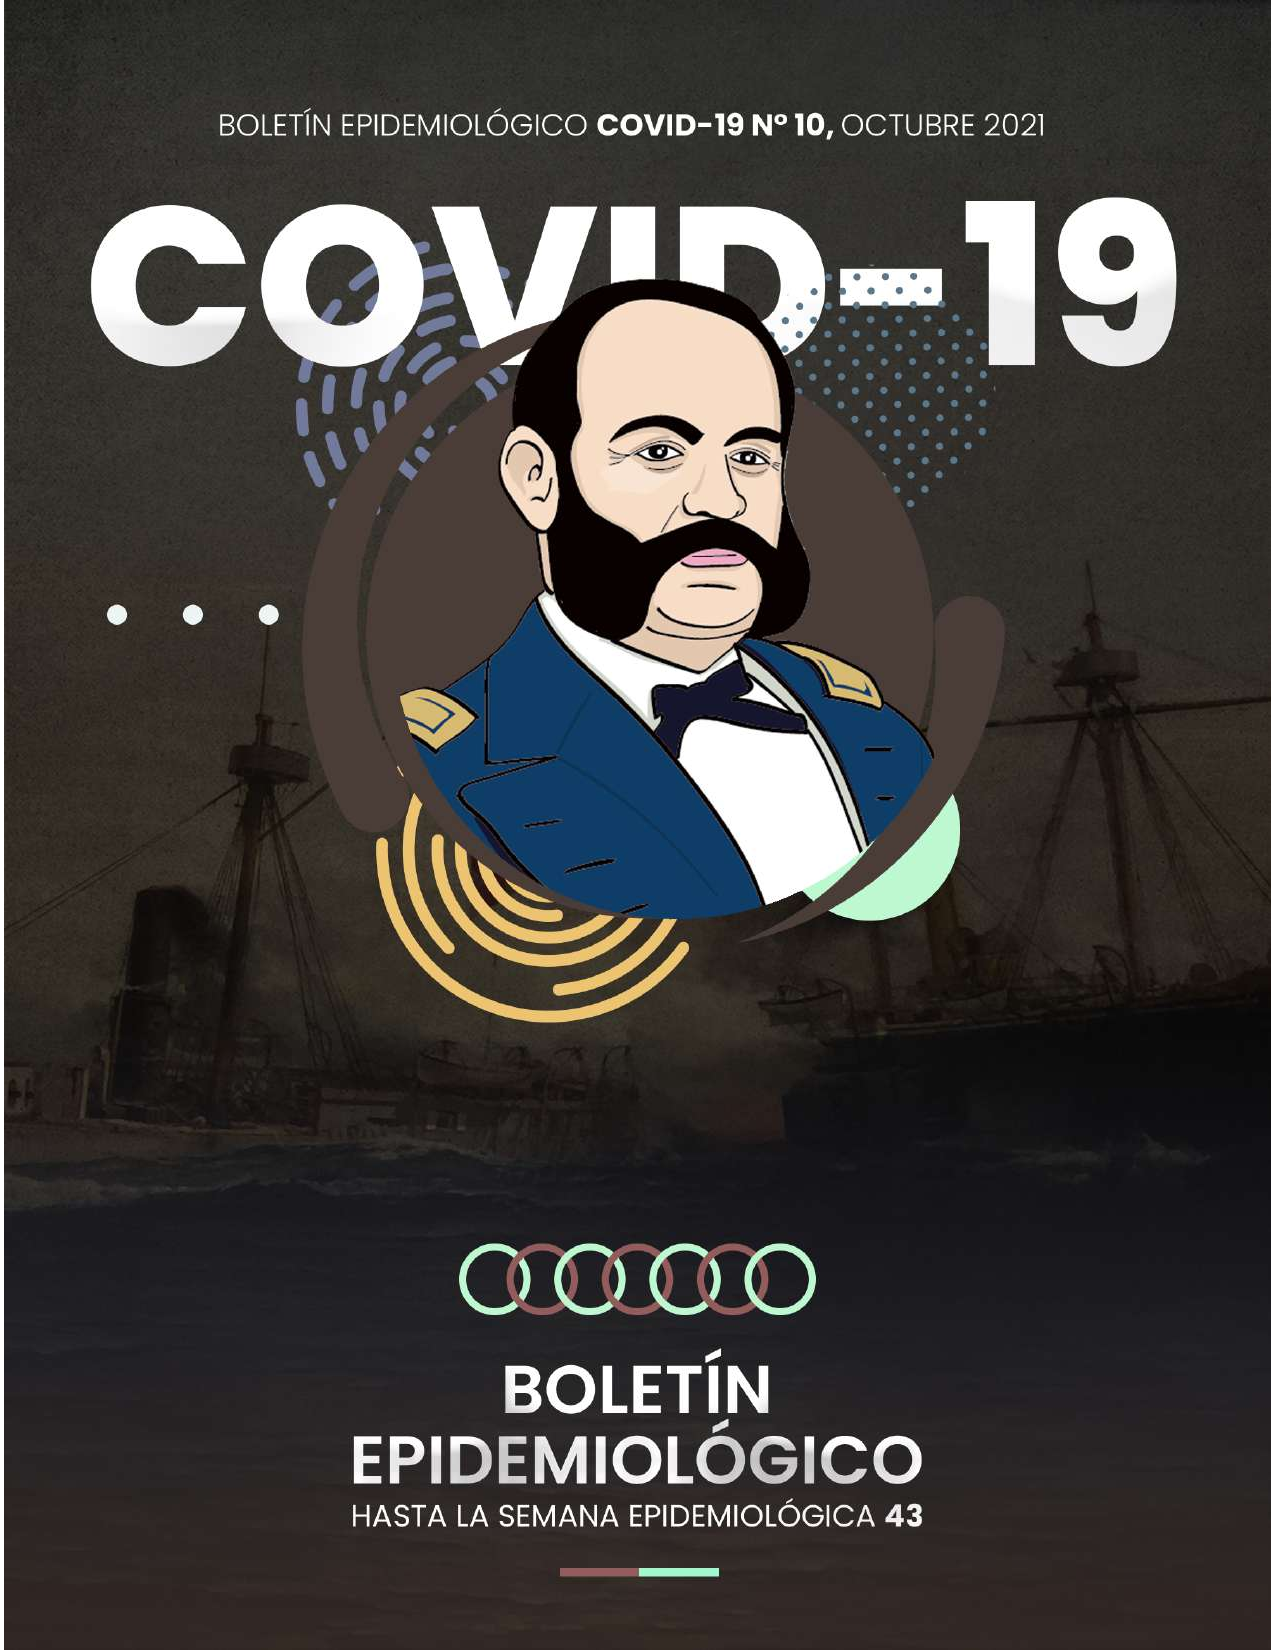
\includepdf[pages={1}]{../editorial/portada.pdf}
	\clearpage
	
	\pagestyle{plain}\pagenumbering{arabic}
	
	\clearpage
	
	
	\begin{center}
	
		{\large Gerencia Regional de Salud}
		
		\textbf{MSP. Javier Ramírez Escóbar}
		
		Gerente Regional \vspace{1.0cm}
		
		Dirección Ejecutiva de Inteligencia Sanitaria
		
		\textbf{MSP. Darío Francisco Navarro Mendoza}
		
		Director
		
		\vspace{1.5cm}
\noindent
\begin{minipage}[t]{.45\textwidth}
	\centering
	Dirección de Epidemiología e Investigación  \\
	\textbf{MSC. Fátima R. Concha Velasco}\\
	Directora \vspace{1.0cm}\\
	% Por orden alfabético del apellido
	\textit{Equipo de Epidemiología e Investigación }\vspace{.5cm}\\
	Econ. Karen Yorka Aguilar Zuñiga \\
	Lic. Nadia Isabel Cáceres Pillco \\
	TAP. Edgar Waldo Capcha Salcedo \\
	M.S.P. Pablo Fidel Grajeda Ancca \\
	M.C. Alex Jaramillo Corrales \\ 
	M.C. Katia Luque Quispe \\
	M.C. Ana Gabriela Eulalia Moncada Arias \\
	M.C. Jesus Kevin Perez Castilla \\
	Lic. Enf. Ruth Nelly Oscco Abarca \\
	Ing. Joel Wilfredo Sumerente Ayerbe \\
	Lic. Enf. Guinetta Margarita Yabar Herrera \vspace{1.5cm}\\	
\end{minipage}
\hfill
\noindent
\begin{minipage}[t]{.45\textwidth}
	\centering
	Dirección de Estadística, Informática y Telecomunicaciones\\
	\textbf{Ing. Abel Rimasca Chacón} \\
	Director \vspace{1.0cm} \\
	% Por orden alfabético del apellido
	\textit{Equipo de Estadística, Informática y Telecomunicaciones} \vspace{.5cm} \\
	Ing. Iván Atayupanqui Rondón \\
	Ing. Miguel Ángel Campana Alarcón \\
	Ing. Uriel Lacuta Farfán \\
	Ing. Jorge Fernando Lovatón Ramos \\
	Ing. Danny Robert Moscoso Sánchez \\
	Lic. Ray Milton Valderrama Álverez \vspace{1.5cm}\\
\end{minipage}
Secretaria: Sra. Ruth Baca Mendoza
	\end{center}
\let\cleardoublepage\clearpage
	\tableofcontents
\begin{center}
Visite nuestro Dashboard interactivo sobre COVID-19 haciendo clic \href{https://geresacusco.shinyapps.io/DASHBOARD\_COVID-19\_CUSCO/}{AQUÍ}
\end{center}
	
	%\mainmatter
	%---------------------------------------------------------------------------
	% CAPÍTULO: EDITORIAL
	%---------------------------------------------------------------------------

	\pagebreak
	
	\section*{Editorial}	\addcontentsline{toc}{chapter}{Editorial}
	\begin{wrapfigure}{l}{8.5cm}
		\label{wrap-fig:1}
		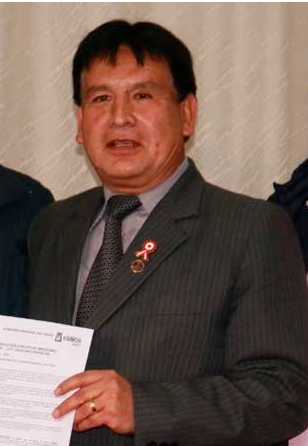
\includegraphics[width=8.5cm]{../editorial/editorial_navarro}
		\caption*{
			\centering
				MC Dario Navarro Mendoza			
				\textit{- Director de Inteligencia Sanitaria-GERESA Cusco.}
				
				 }
	\end{wrapfigure}
	
	\noindent \textbf{La Pandemia en la era de Ómicron}
	

En el contexto actual de la tercera ola de la Pandemia por COVID-19, con un aumento acelerado en el número de casos, con predominio de la variante ómicron, ha generado un incremento en la demanda de pruebas diagnósticas, que supera a la demanda de vacunas, obligando al sistema de salud a incrementar los puntos de toma de muestra o los llamados puntos COVID-19. Paralelamente en los Hospitales existe una congestión en sus servicios tanto el área COVID-19 como en el área no COVID-19, incorporándose en esta demanda la población infantil afectada por esta enfermedad, fenómeno que antes no se había observado.
Ante este escenario es importante el papel que desempeña el primer nivel de atención para la contención de casos leves y moderados, que es la mayor parte de la población demandante, siendo necesario el fortalecimiento en dos acciones importantes: primero la captación y diagnóstico oportuno y segundo en fortalecer los cuidados en casa de pacientes positivos, así como la cuarentena efectiva de los contactos directos. Es así, que es necesario prestar atención a las actividades comunicacionales con contenidos sobre la identificación de signos y síntomas de alarma de COVID-19, conocer la población más vulnerable para evitar el contagio intradomiciliario y afección de los más vulnerables. Por lo cual, es necesario prestar atención a la burbuja familiar, ambientes ventilados y acciones de control y fiscalización por parte de los Comandos COVID-19 provinciales y distritales.
Debido a las características de la variante ómicron, como la alta infectividad (transmisibilidad) y baja letalidad, el escenario de “lucha” contra la Pandemia del COVID-19 se está trasladando hacia un escenario en el cual el fortalecimiento de la comunicación y acciones preventivas dependen de la comunidad. Por lo que, es necesario e importante continuar con el cierre de brechas en la vacunación tanto de primera, segundas y el refuerzo de la tercera dosis.	
	
	%---------------------------------------------------------------------------
	% CAPÍTULO: METODOLOGÍA
	%---------------------------------------------------------------------------
			%insertar el cover del capitulo
	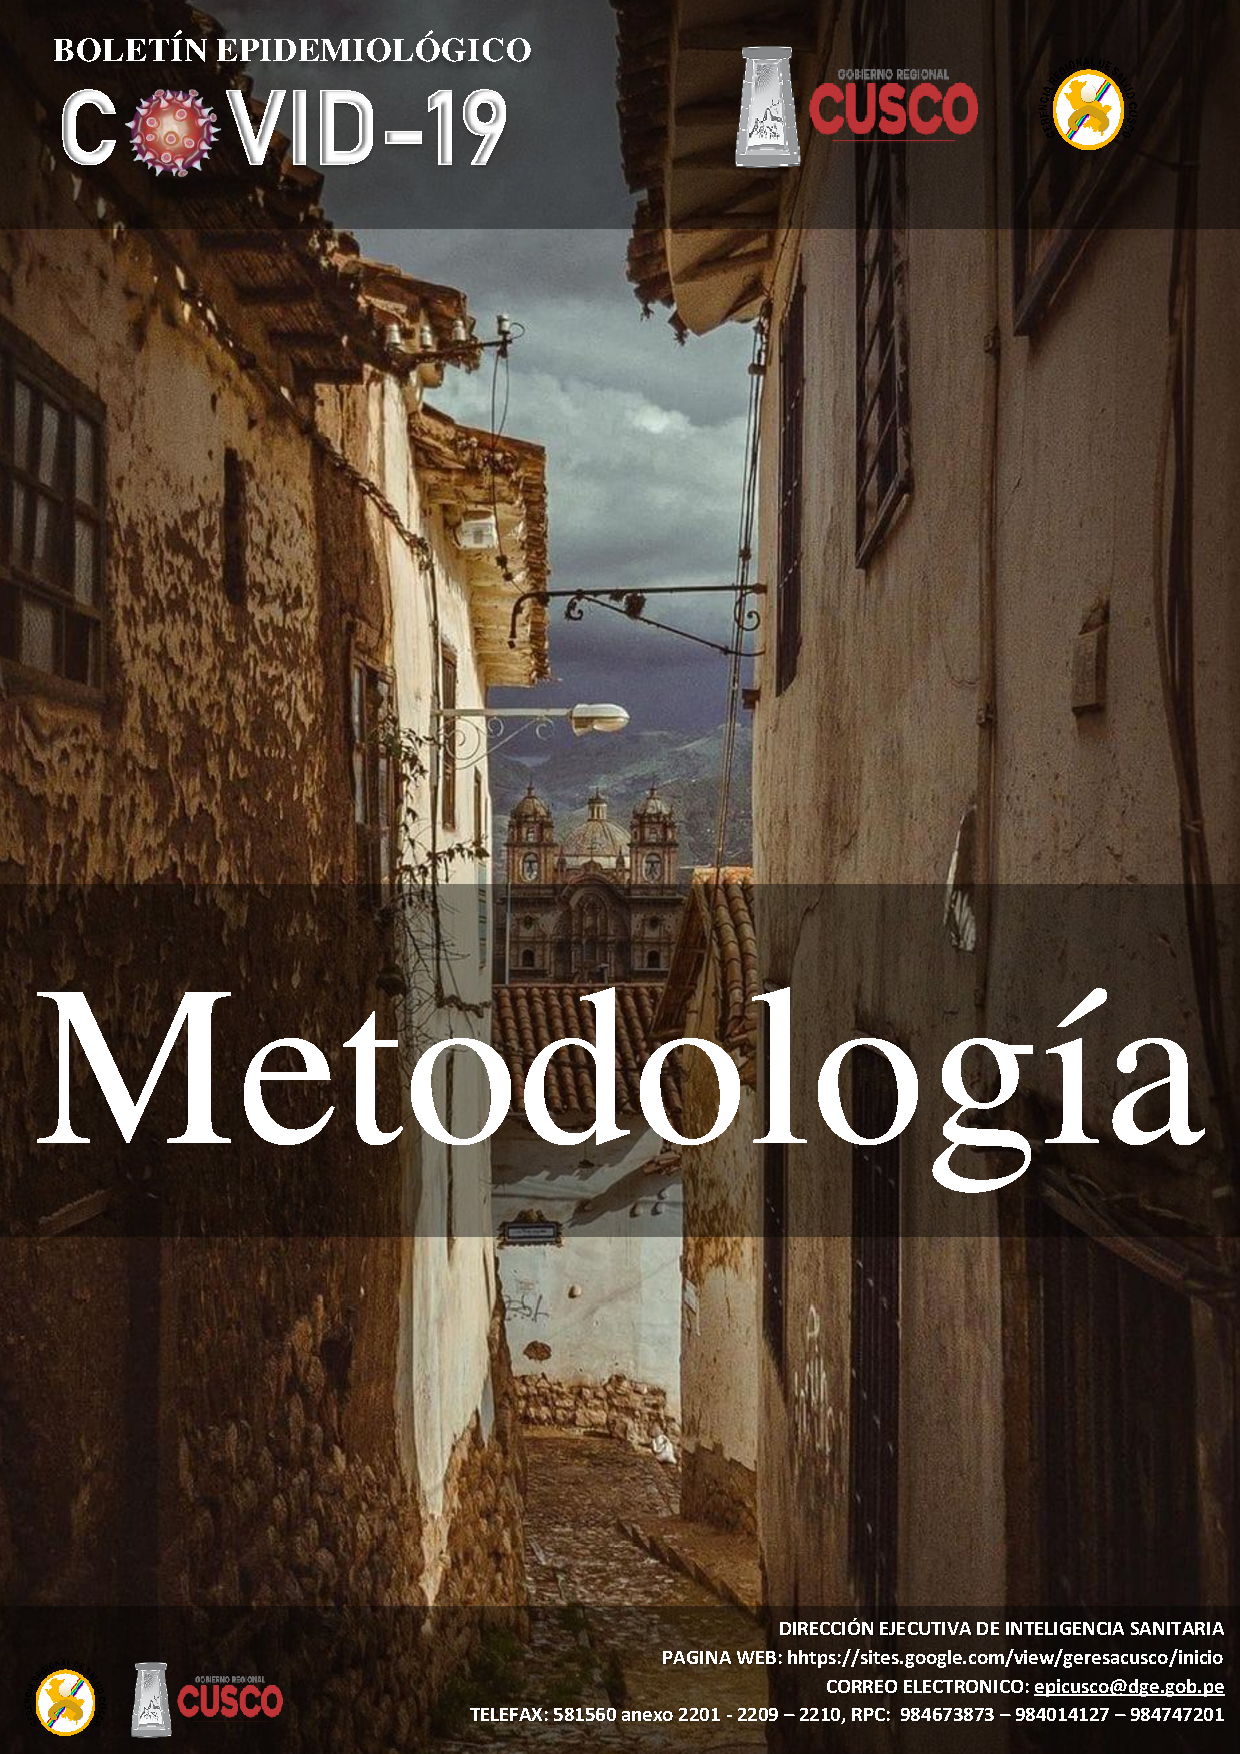
\includepdf[pages={1}]{../editorial/1.pdf}
	\clearpage
	
	\section*{Metodología}	
	\addcontentsline{toc}{chapter}{Metodología}
	\noindent El presente Boletín tiene el objetivo de informar sobre los principales indicadores epidemiológicos y de gestión hospitalaria,  para hacer el seguimiento de la pandemia en nuestra región y tomar mejores decisiones. Este Boletín tiene una metodología de tipo descriptiva. 
	
	La introdución de la variante ómicron en nuestra región ha marcado el inicio de la tercera ola pandémica, es por esto que en esta edición del boletín se considera los datos desde el año 2021 hasta la semana epidemiológica 3 (22 de enero del 2022), para que el lector pueda hacer las comparaciones e inferencia del comportamiento de la segunda ola y la ola actual por la que atraviesa nuestra región. Asimismo, en la descripción de cada indicador o figura se indicará si el análisis de la información incluye otro periodo. 
	
	Los datos analizados incluyeron: a) características generales: sexo, edad, casos confirmados, fallecidos; b) características clínicas: síntomas reportados, casos confirmados sintomáticos, casos confirmados asintomáticos y comorbilidades; c) indicadores epidemiológicos: sistema de vigilancia epidemiológica, tasa de mortalidad, tasa de positividad de pruebas diagnósticas, casos activos – recuperados, y exceso de muerte por todas las causas, y d) indicadores de gestión hospitalaria: , ocupación de camas UCI y No UCI en la Región. En este boletín se considera como caso positivo de COVID-19, sólo a aquellos que tienen una prueba antigénica o molecular positiva, salvo en ciertas estimaciones, en cuya descripción se detalla si se utilizó otro tipo de examen diagnóstico. 
	
	Las fuentes de información son las bases de datos de NOTI WEB (aplicativo del Sistema de Vigilancia Epidemiológica - COVID-19), SISCOVID (Sistema Integrado para COVID-19), SINADEF (Sistema Informático Nacional de Defunciones), SICOVAC-HIS MINSA(Base de datos de vacunación por COVID-19), Reporte de Disponibilidad de Camas de Hospitalización y datos de la Oficina de Referencias-Contrarreferencias de la Dirección de Emergencias y Desastres de GERESA-Cusco. 
	
	Se usaron frecuencias absolutas y relativas para la descripción de los datos cualitativos. Para la descripción de datos cuantitativos se calcularon tasas (mortalidad, pruebas diagnósticas, incidencia de casos), promedios (ocupación de camas hospitalarias, fallecidos por COVID y fallecidos por todas las causas). Para describir la tendencia se representaron los datos cuantitativos y frecuencias relativas en intervalos de 7 días (semana epidemiológica). En las variables de sistema de vigilancia epidemiológica (1 prueba por 100,000 habitantes) y ocupación de cama (adecuado, menor a $70\%$, moderado, entre $75$ a $90\%$ y limitado, más de $90\%$), siendo todos los puntos de referencia sugeridos por la Organización Mundial de la Salud. Para el análisis de exceso de mortalidad, se usó la metodología descrita por C. Giattino, H. Ritchie, M. Roser, E. Ortiz-Ospina, y J. Hasell en el artículo "Excess mortality during the Coronavirus pandemic (COVID-19)". Published online at OurWorldInData.org.
	
	La descripción de dichas variables se hace de manera regional y provincial. En la presente edición se hace una descripción de la tasa de incidencia, tasa de mortalidad, tasa de positividad por prueba molecular y antigénica, y exceso de defunciones de todas las provincias de nuestra región. El lector interesado en un análisis distrital de los casos y defunciones puede encontrar dicha información en los links correspondientes.
	 
	%---------------------------------------------------------------------------
	% CAPÍTULO: CARACTERÍSTICAS GENERALES
	%---------------------------------------------------------------------------
		%insertar el cover del capitulo
	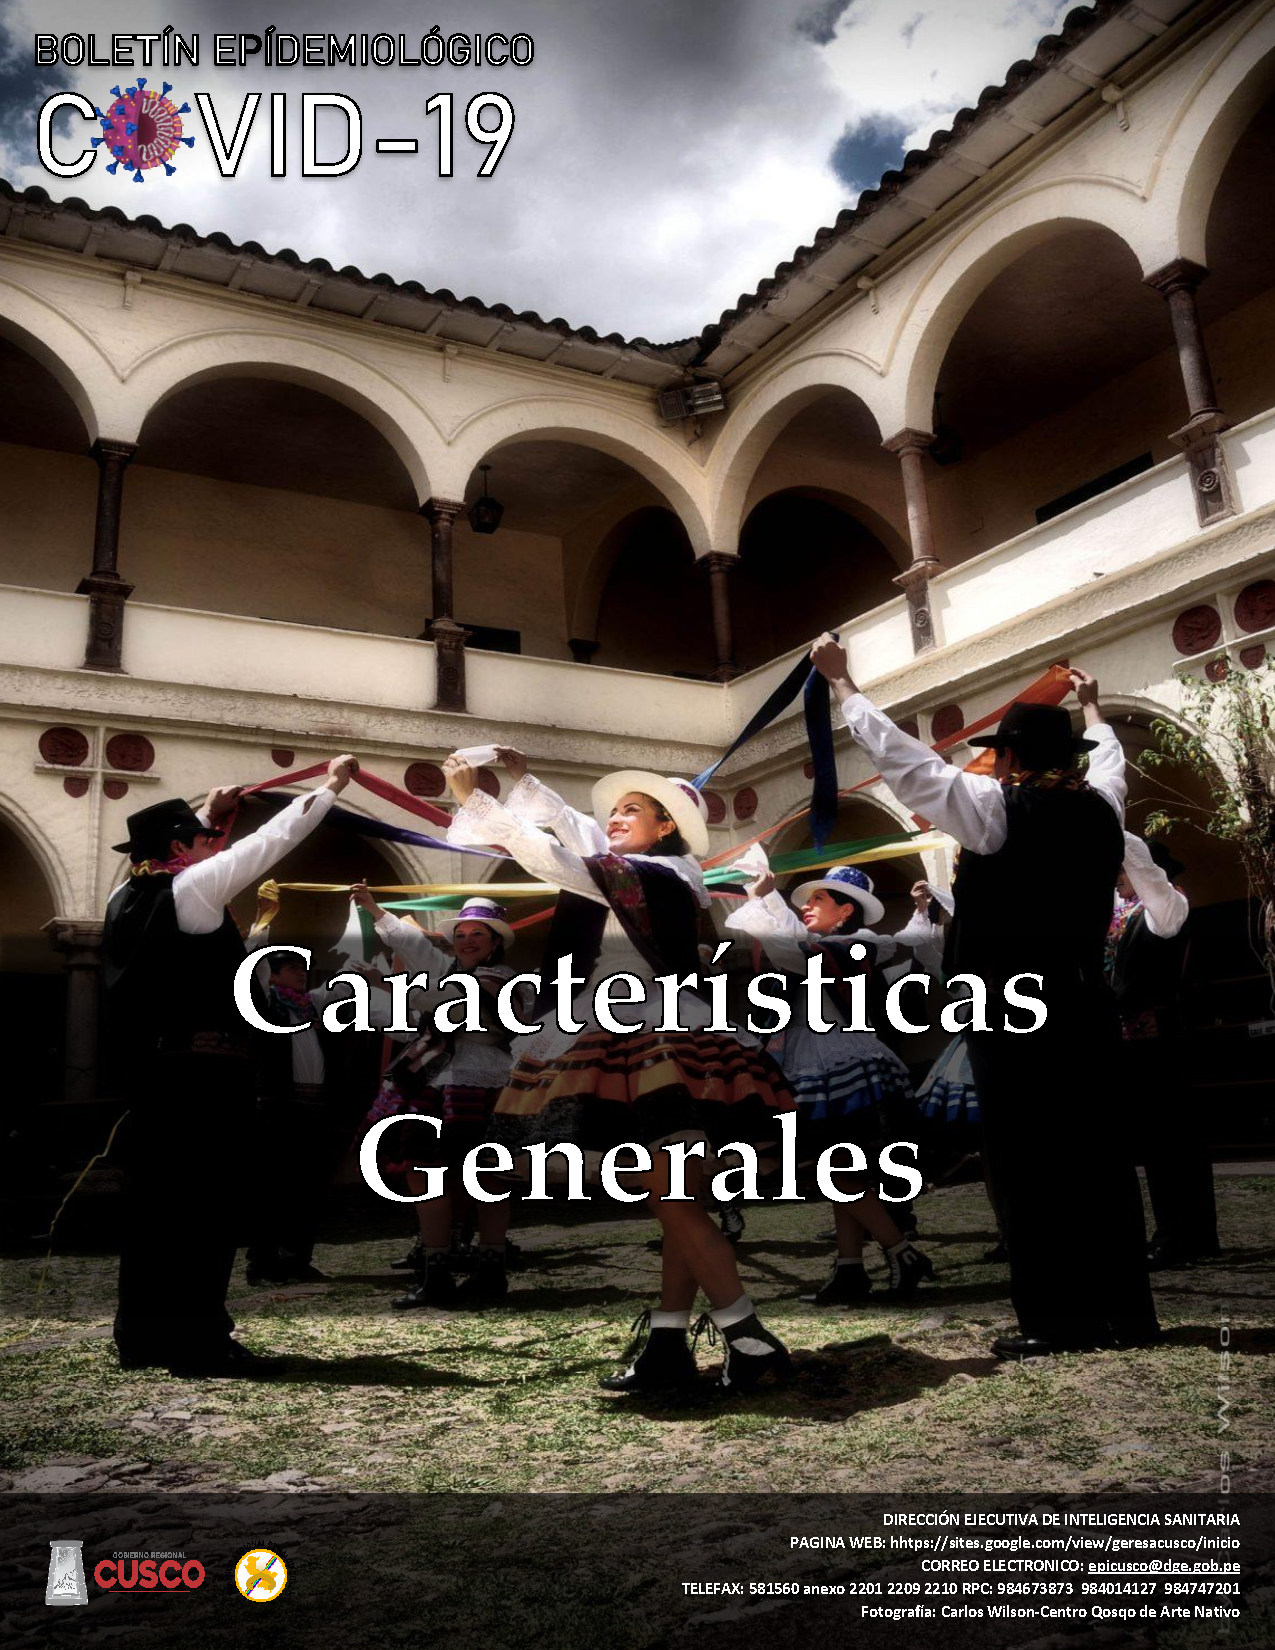
\includepdf[pages={1}]{../editorial/2.pdf}
	\clearpage	
	\section*{Características Generales}
	\addcontentsline{toc}{chapter}{Características Generales}
	
	
	
 	\noindent En la Figura \ref{fig:casos_edad_sexo} se muestra la cantidad de casos confirmados de COVID-19, por prueba antigénica o molecular por grupo etario (en intervalos de 10 años) y sexo. Se observa que la mayor cantidad de casos diagnosticados hasta la SE 03, se concentra en el grupo etario de 30 a 39 años(7284 casos acumulados), con mayor afectación del sexo femenino, seguido del grupo etario de 20 a 29 años (7000 casos acumulados) con mayor afectación del sexo femenino. Es importante recalcar que la cantidad de niños afectados de 0 a 9 años (562 casos acumulados) es la mayor que se registra en toda la pandemia. 
 	
 	
\begin{figure}[h]
	\caption{Casos Confirmados de COVID-19 según Grupo de Edad y Sexo en la Región Cusco hasta la SE 07-2022(*).}\label{fig:casos_edad_sexo}
	\begin{center}
		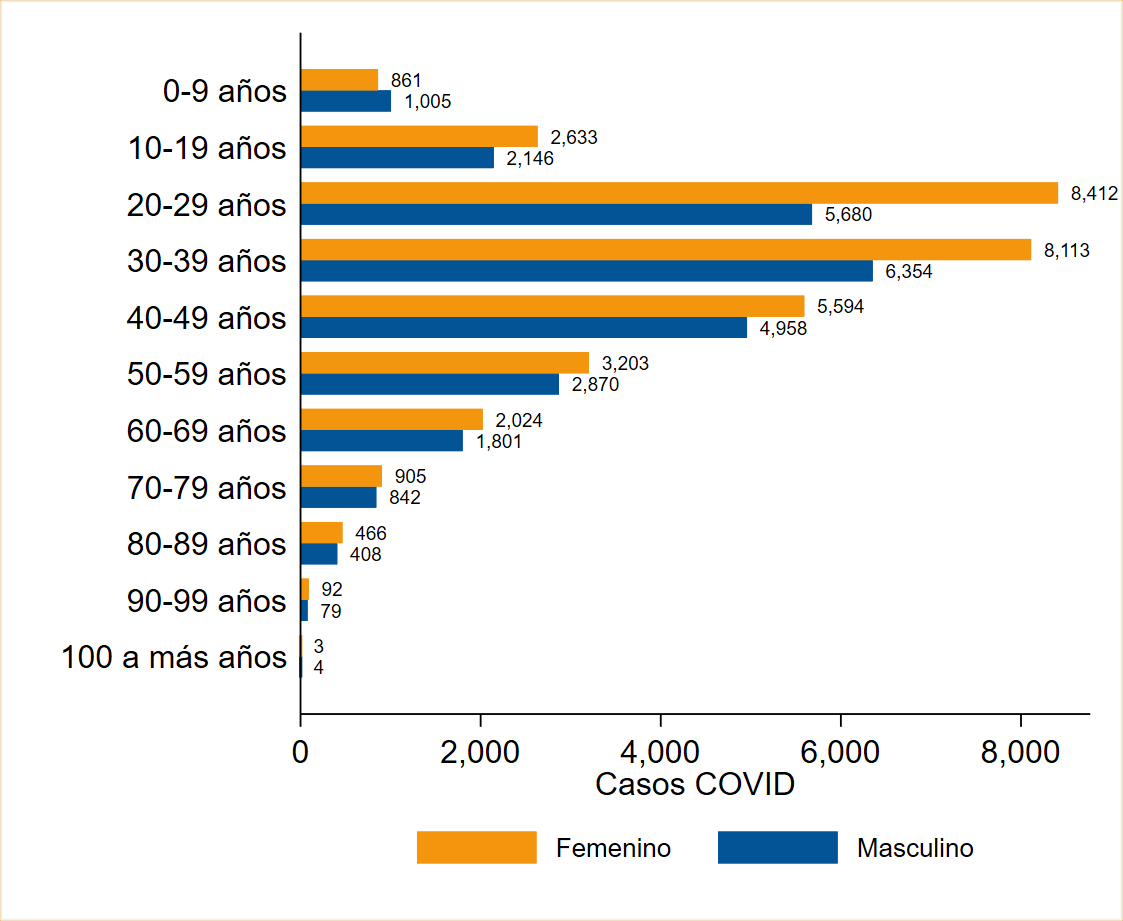
\includegraphics[width=0.75\linewidth]{../figuras/casos_etapavida_2022}
	\end{center}
	{\footnotesize {Fuente de datos: SISCOVID, NOTICOVID.(*)Sólo se incluye información del 2022.}}
\end{figure}
\pagebreak


La Figura \ref{fig:fallecidos_edad_sexo}  muestra el número de muertes reportadas por COVID-19 conforme al grupo etario y sexo hasta el 22 de enero del 2022, se observa que el mayor número de muertes se registra en el grupo etario de 80 a 89 años (16 muertes acumuladas), con mayor afectación del sexo masculino, seguido del grupo etario de 70 a 79 años (7 muertes acumuladas). 

\begin{figure}[h]
	\caption{Casos fallecidos por COVID-19 según Grupo Etario y Sexo en la Región Cusco hasta la SE 07-2022(*).}\label{fig:fallecidos_edad_sexo}
	\begin{center}
		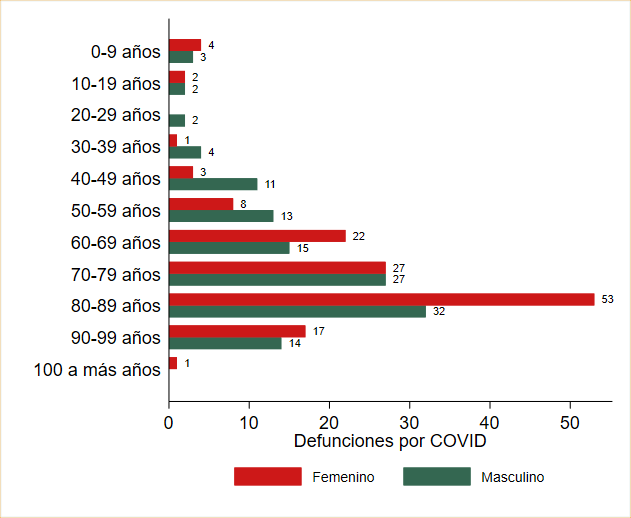
\includegraphics[width=0.75\linewidth]{../figuras/defunciones_etapavida_2022}
	\end{center}
	{\footnotesize {Fuente de datos: SISCOVID, NOTICOVID.(*)Sólo se incluye información del 2022.}}
\end{figure}



\cleardoublepage
%---------------------------------------------------------------------------
% CAPÍTULO: CARACTERÍSTICAS CLÍNICAS
%---------------------------------------------------------------------------
	%insertar el cover del capitulo
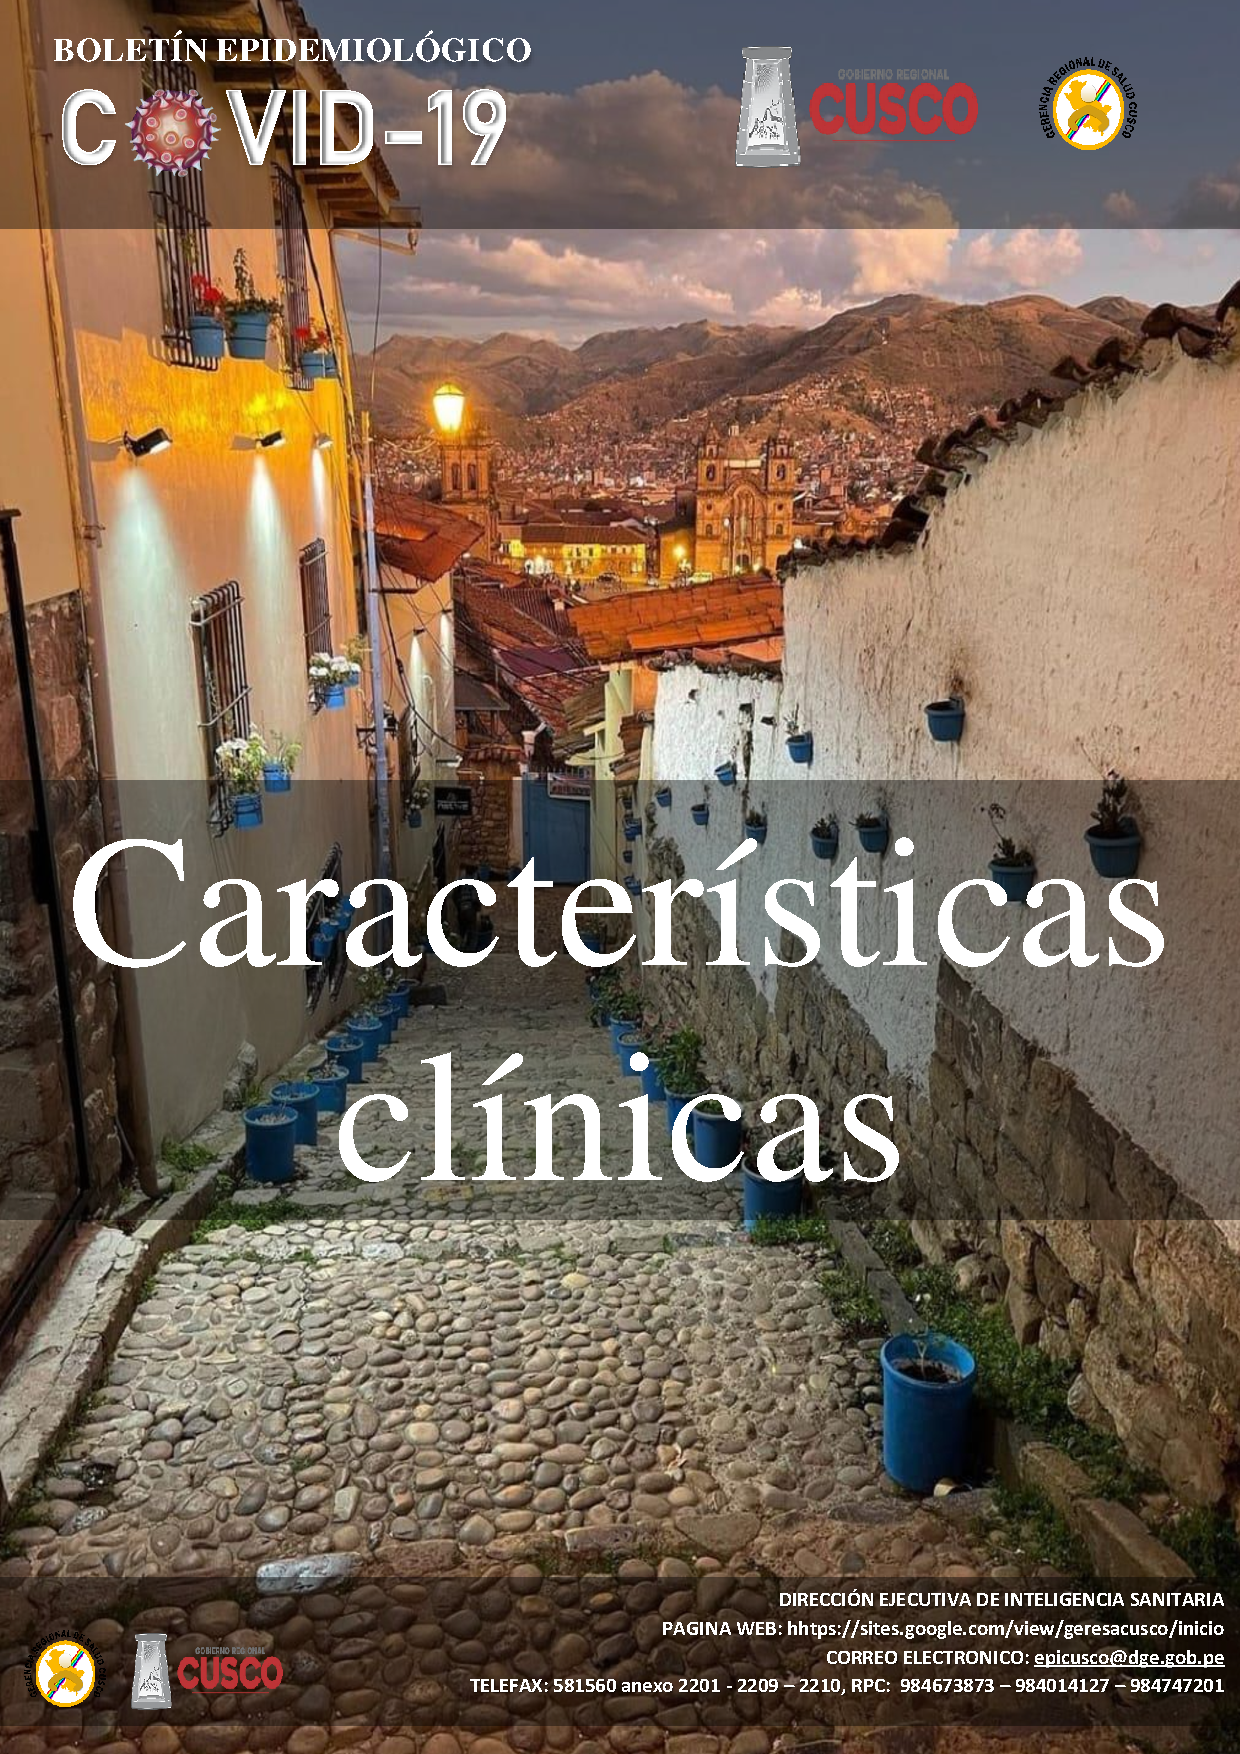
\includepdf[pages={1}]{../editorial/3.pdf}

\clearpage

\section*{Características Clínicas}
\addcontentsline{toc}{chapter}{Características Clínicas}	


\noindent En la Figura \ref{fig:sintomas}, se presentan los síntomas más frecuentes autorreportados por los pacientes con diagnóstico de COVID-19, el dolor de garganta (18,7 $\%$) es el síntomas más reportado, seguido de tos (17,3 $\%$) y malestar (13,5$\%$). Dentro de los signos (Figura \ref{fig:signos}) más frecuentes el exudado faríngeo constituye el signo más prevalente (89,8$\%$). 

\begin{figure}[h]
	\caption{Síntomas más frecuentes de los pacientes diagnosticados por COVID-19 en la Región Cusco hasta la SE 07-2022.  }\label{fig:sintomas}
	\begin{center}
		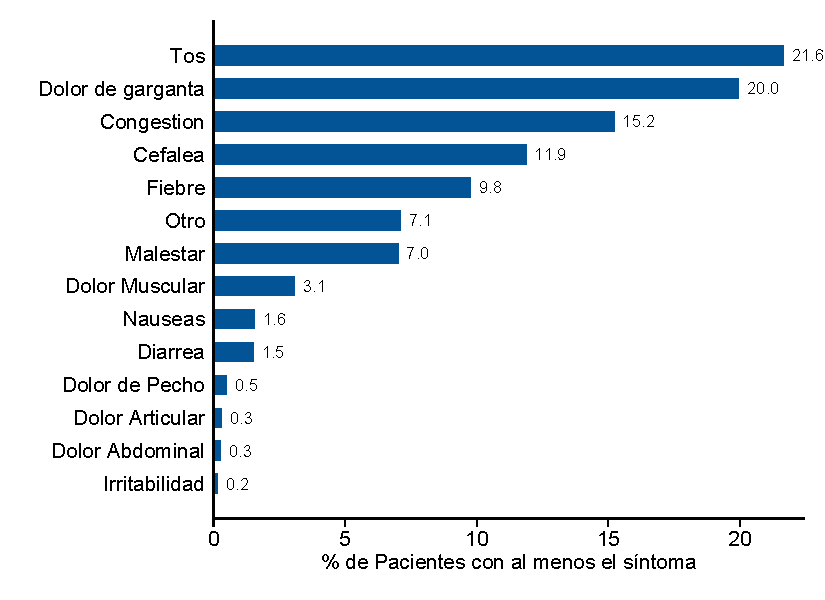
\includegraphics[width=0.85\linewidth]{../figuras/figura_sintoma.pdf}
	\end{center}
	{\footnotesize {Fuente de datos: SISCOVID, NOTICOVID.}}
\end{figure}

\begin{figure}[h]
	\caption{Signos más frecuentes de los pacientes diagnosticados por COVID-19 en la Región Cusco hasta la SE 07-2022.}\label{fig:signos}
	\begin{center}
		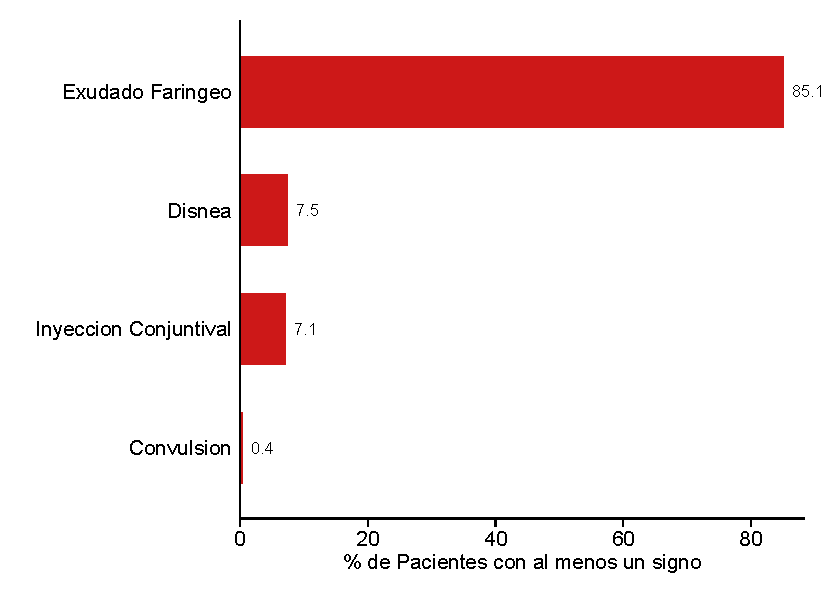
\includegraphics[width=0.65\linewidth]{../figuras/figura_signo.pdf}
	\end{center}
	{\footnotesize {Fuente de datos: NOTICOVID.}}
\end{figure}

La Figura \ref{fig:comorbilidades} muestra la frecuencia de comorbilidades autoreportadas por los pacienteS con COVID-19, siendo las más prevalentes la obesidad (32,5$\%$), diabetes (32,5$\%$) y las comorbilidades cardiovasculares (32,5$\%$).  
\begin{figure}[h]
	\caption{Comorbilidades más frecuentes de los pacientes diagnosticados por COVID-19 en la Región Cusco hasta la SE 07-2022. }\label{fig:comorbilidades}
	\begin{center}
		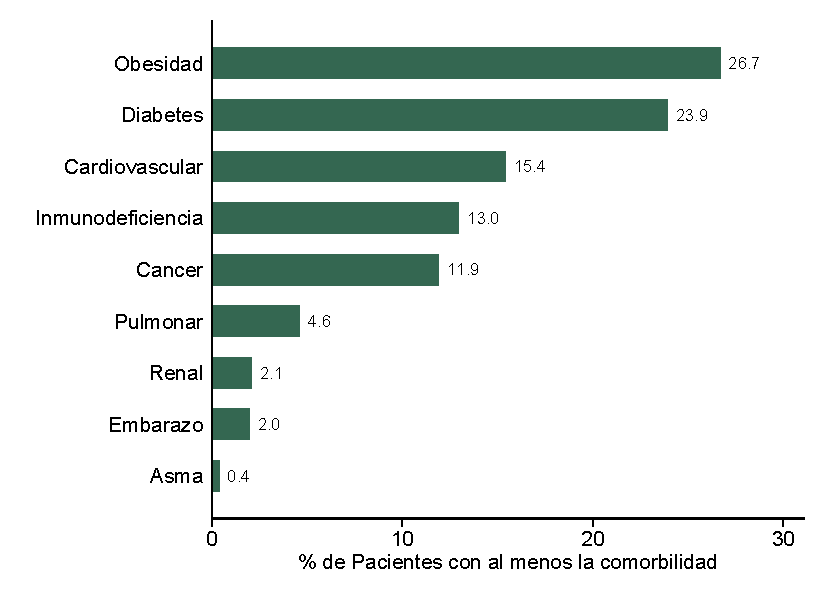
\includegraphics[width=0.65\linewidth]{../figuras/figura_comorbilidad.pdf}
	\end{center}
	{\footnotesize {Fuente de datos: NOTICOVID.}}
\end{figure}
\clearpage
 En la Figura \ref{fig:sintomaticos_asintomati} se evidencia la curva epidémica de casos sintomáticos y asintomáticos detectados por pruebas moleculares y antigénicas, comparada con los casos sintomáticos y asintomáticos desde el año 2020. Para el año 2022, se evidencia un marcado incremento tanto de los casos asintomáticos como los síntomáticos, con una pendiente en ascenso sostenido.  
 
\begin{figure}[h]
	\caption{Casos Sintomáticos y Asintomáticos de COVID-19 por Semana Epidemiológica en la Región Cusco, hasta la SE 07-2022.  }\label{fig:sintomaticos_asintomati}
	
	\begin{center}
		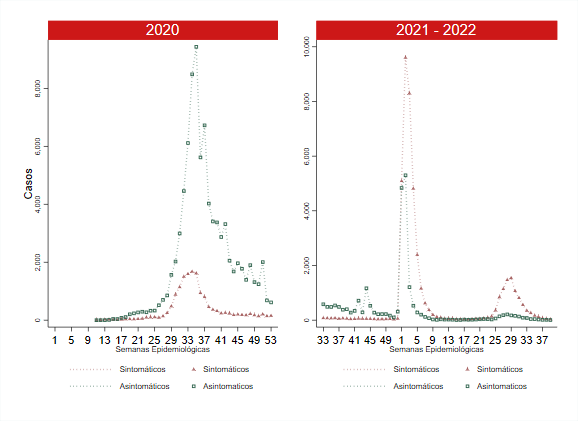
\includegraphics[width=0.75\linewidth]{../figuras/sintomaticos_20_21_22.png}
	\end{center}
	{\footnotesize {Fuente de datos: SISCOVID, NOTICOVID.}}
\end{figure}
\clearpage


%---------------------------------------------------------------------------
% CAPÍTULO: ANÁLISIS DE INDICADORES
%---------------------------------------------------------------------------
%insertar el cover del capitulo
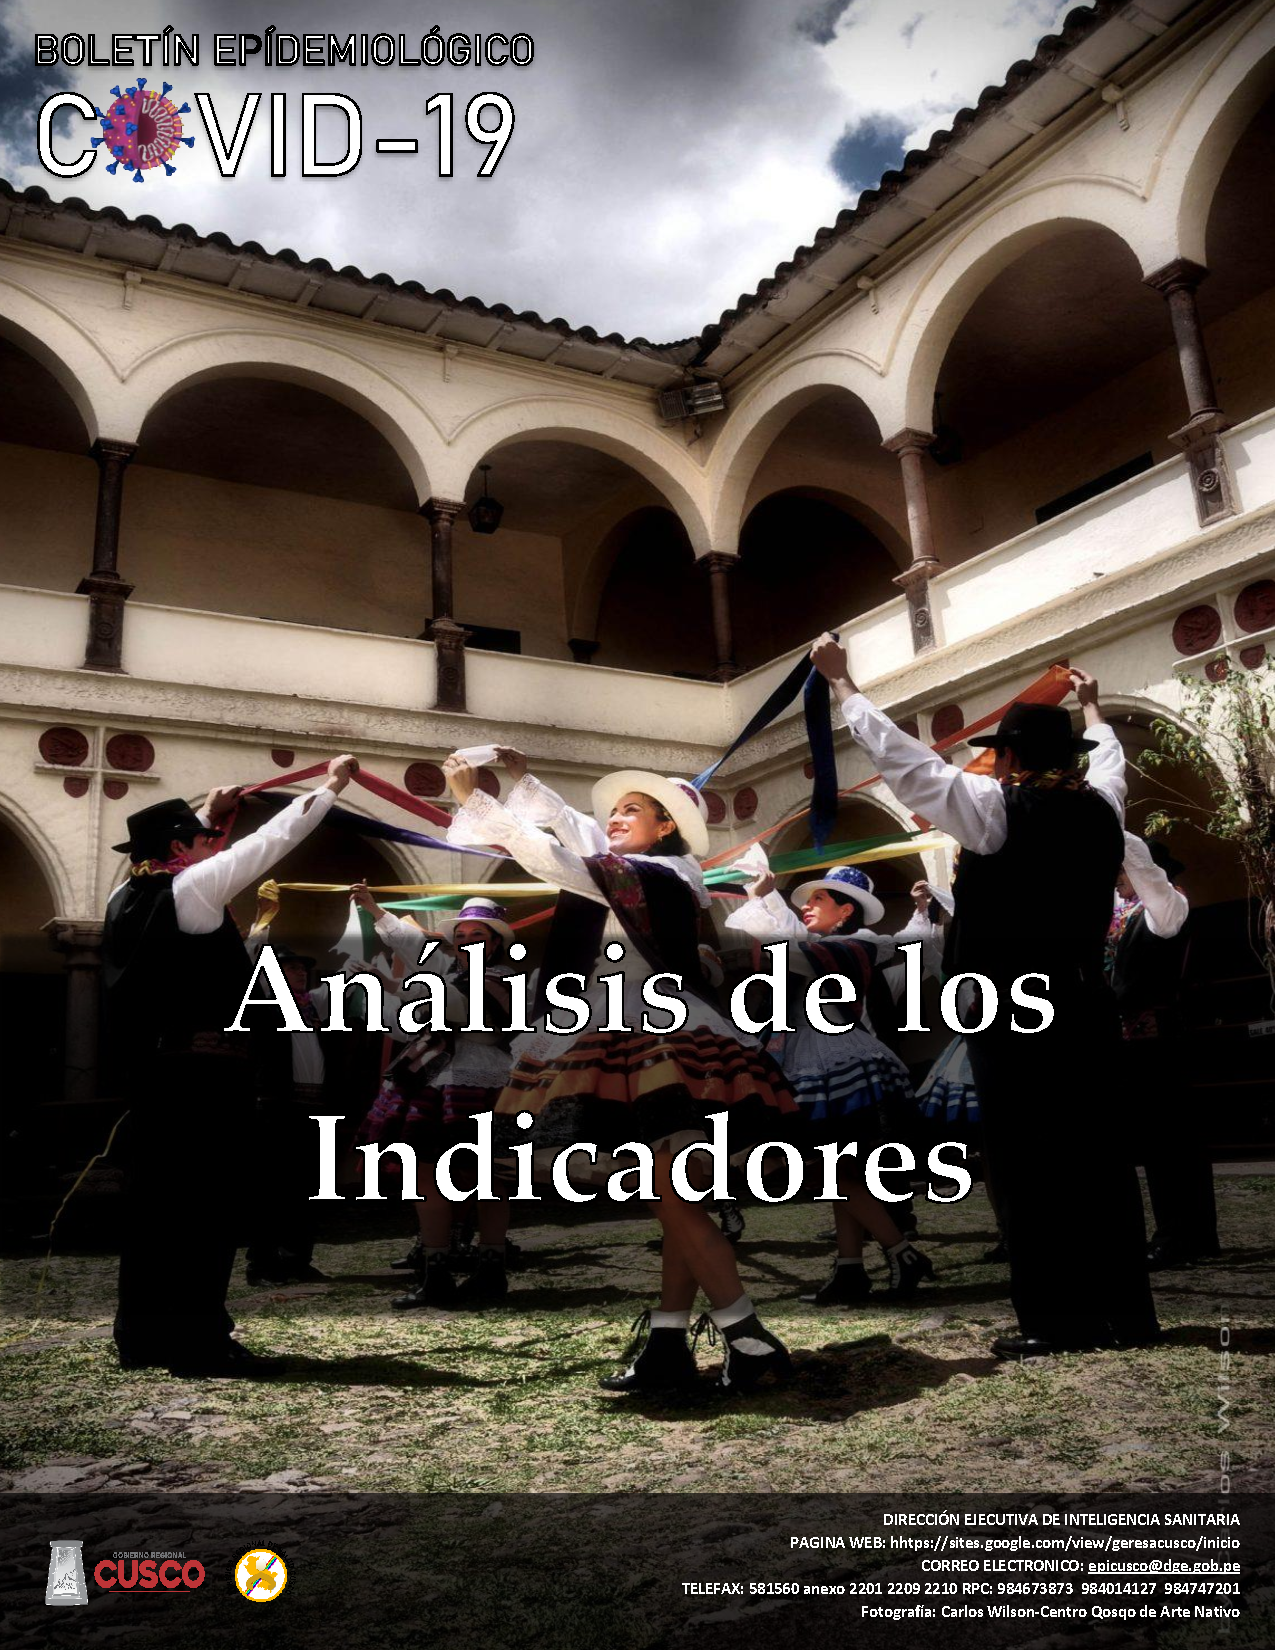
\includepdf[pages={1}]{../editorial/4.pdf}
\clearpage

    \section*{Análisis de Indicadores}
    \addcontentsline{toc}{chapter}{Análisis de Indicadores}
   	\subsection*{Tasa de Incidencia y Tasa de Positividad}
\noindent La evolución de la tasa de incidencia en el tiempo se encuentra graficada en la Figura \ref{fig:incidencia}, se observa un incremento sostenido de casos durante la SE 01 y 02 del año 2022, alcanzando en la SE 01 del 2022 una tasa de 602 casos/ 1 000 000 personas, cifra mucho más alta que las máximas reportadas en la segunda y primera ola, asimismo la pendiente de crecimiento de la tasa de incidencia continua francamente en ascenso, la variación para la SE 03 queda sujeta al tiempo de demora para la actualización de resultados. 

  \begin{figure}[h]
  	\caption{Tasa de Incidencia de COVID-19 en la región Cusco hasta la SE 07-2022.(*) }\label{fig:incidencia}
  	\begin{center}
  		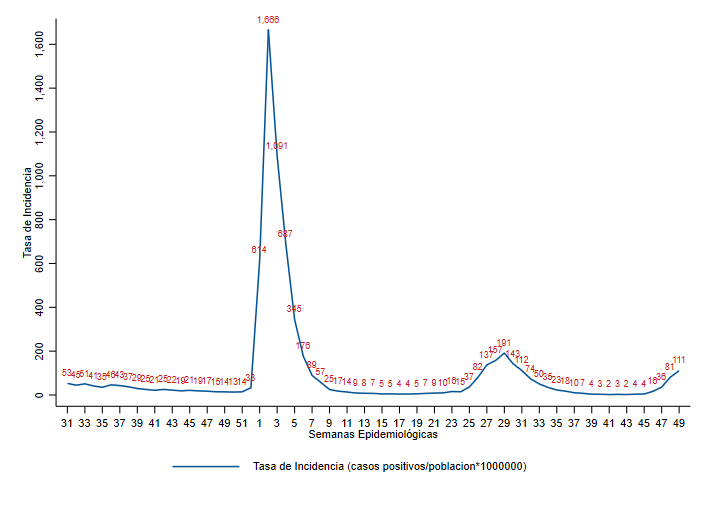
\includegraphics[width=0.80\linewidth]{../figuras/tasa_incidencia_2021_2022.png}
  	\end{center}
  	{\footnotesize {Fuente de datos: SISCOVID, NOTICOVID. (*) Se considera como caso positivo sólo a los pacientes con prueba molecular o antigénica positiva.}}
  \end{figure}
   
  La Figura \ref{fig:total_muestras_procesada} muestra un comparativo de las tasas de positividad ($\%$) de pruebas moleculares (PCR) y antigénicas (AG). La tasa de positividad de ambas pruebas se encuentra en ascenso desde la SE 52 del 2021, en el caso de las pruebas moleculares, en la primera semana del 2022 se reportó el porcentaje máximo de positividad en toda la pandemia (60$\%$), mientras que la positividad de pruebas antigénicas sigue en ascenso sostenido, alcanzando su máximo porcentaje de positividad (46$\%$) en la SE 03. 
  
   \begin{figure}[h]
	\caption{Tasa de positividad para muestras antigénicas y moleculares por COVID-19 en la región Cusco hasta la SE 07-2022. }\label{fig:total_muestras_procesada}
	\begin{center}
		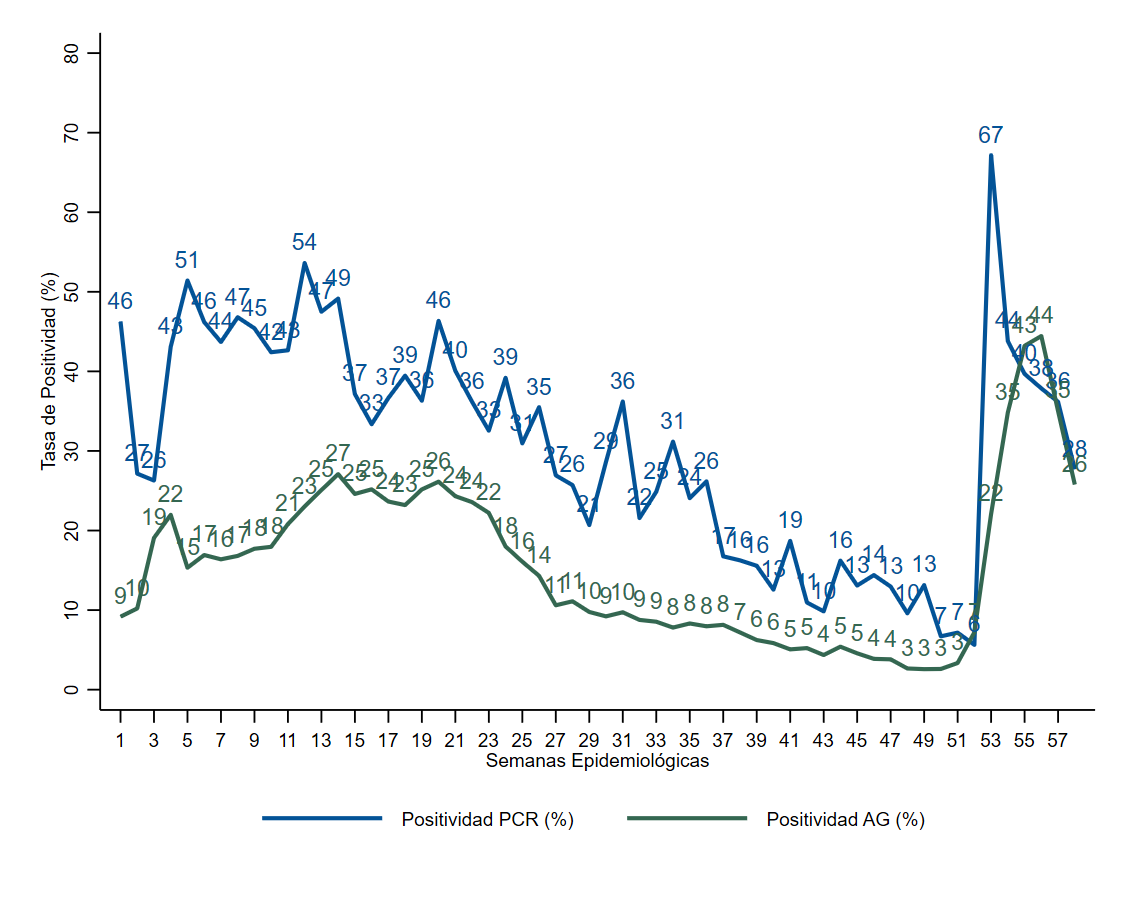
\includegraphics[width=0.75\linewidth]{../figuras/positividad_diaria_2021_2022.png}
	\end{center}
	{\footnotesize {Fuente de datos: SISCOVID, NOTICOVID.}}
\end{figure}


La Figura \ref{fig:positividad_pcr} muestra el número de pacientes detectados por cada prueba, junto con una comparación de la tasa de positividad por semana, es evidente que el número de pruebas realizadas y la tasa de positividad han ido incrementando desde la SE 52 del 2021. La Figura \ref{fig:positividad_ag}
muestra la situación de la pruebas antigénicas, se aprecia un marcado incremento en el número de pruebas positivas desde la SE 52.   

\begin{landscape}
	\begin{figure}[h]
		\caption{Positividad y Tasa de Positividad de pruebas moleculares tomadas por COVID-19 en la región Cusco hasta la SE 07-2022.}\label{fig:positividad_pcr}
		\begin{center}
			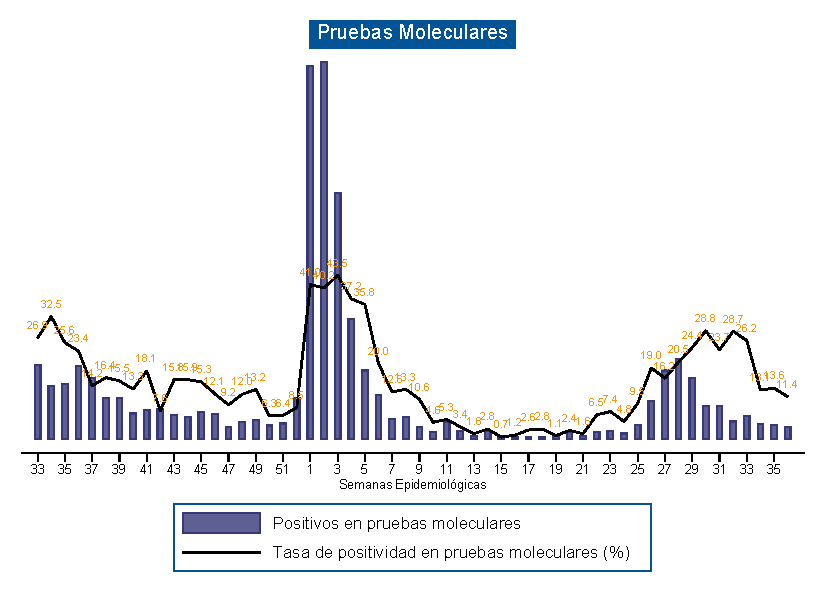
\includegraphics[width=0.90\linewidth]{../figuras/positividad_pcr.pdf}
		\end{center}
		{\footnotesize {Fuente de datos: SISCOVID, NOTICOVID.}}
	\end{figure}
\end{landscape}
\clearpage
\begin{landscape}

	\begin{figure}[h]
		\caption{ Positividad y Tasa de Positividad de pruebas antigénicas tomadas por COVID-19 en la región Cusco hasta la SE 07-2022.}\label{fig:positividad_ag}
		\begin{center}
			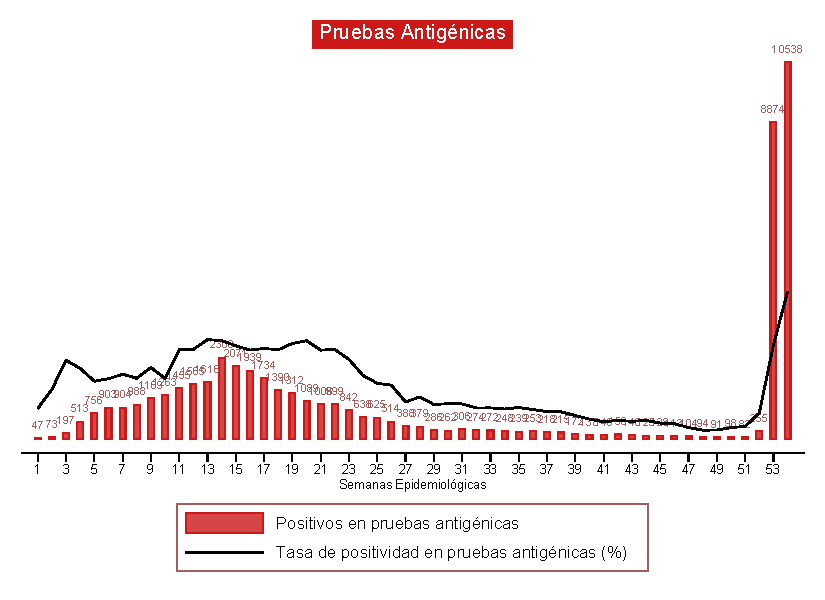
\includegraphics[width=0.90\linewidth]{../figuras/positividad_ag.pdf}
		\end{center}
		{\footnotesize {Fuente de datos: SISCOVID, NOTICOVID.}}
	\end{figure}
\end{landscape}
\clearpage


	\subsection*{Análisis de la Mortalidad}

\noindent En la Figura \ref{fig:mortalidad_edad} se muestra la mortalidad semanal para las edades agrupadas en decenios, donde la línea vertical entrecortada marca el inicio del año 2022. Para la SE 03 del año 2022, existe un aumento de muertes en comparación a las semanas previas, a predominio de los mayores de 80 años, sin embargo la tasa de mortalidad es menor a la reportada en la misma semana del 2021. 
	 	
\begin{figure}[h]
	\caption{Tasa de Mortalidad por COVID-19 por Grupo Etario hasta la SE 07-2022.}\label{fig:mortalidad_edad}
	\begin{center}
		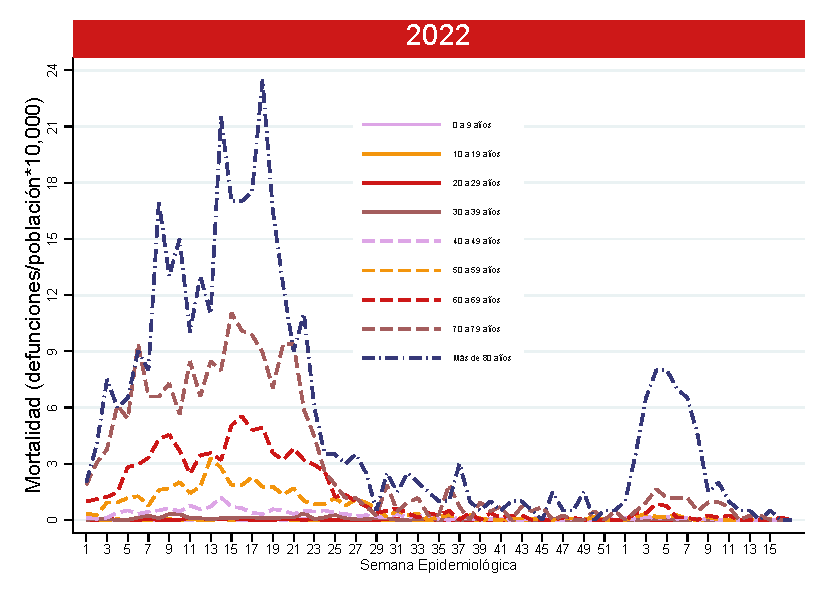
\includegraphics[width=0.65\linewidth]{../figuras/mortalidad_edad_2021_2022.pdf}
	\end{center}
	{\footnotesize Fuente de datos: SINADEF} 
\end{figure}


La Figura \ref{fig:mortalidad_grupo_edad} muestra la relación entre la tasa de mortalidad y la vacunación desde los 30 años. Las líneas de referencia representan las fechas del inicio de la vacunación (primera dosis) para el correspondiente grupo etario y al inicio del año 2022. Se aprecia que para la SE 03 del año 2022 hubo un incremento de muertes en todos los grupos etarios excepto en el grupo de 30 a 39 años. Asimismo aún este incremento de mortalidad por edades es menor a las cifras reportadas en la misma semana del año 2021.  

	\begin{figure}[h]
	\caption{Tasa de Mortalidad por COVID-19 por Grupo Etario hasta la SE 07-2022.}
	\label{fig:mortalidad_grupo_edad}
	\centering
	\begin{subfigure}[b]{0.45\textwidth}
		\centering
		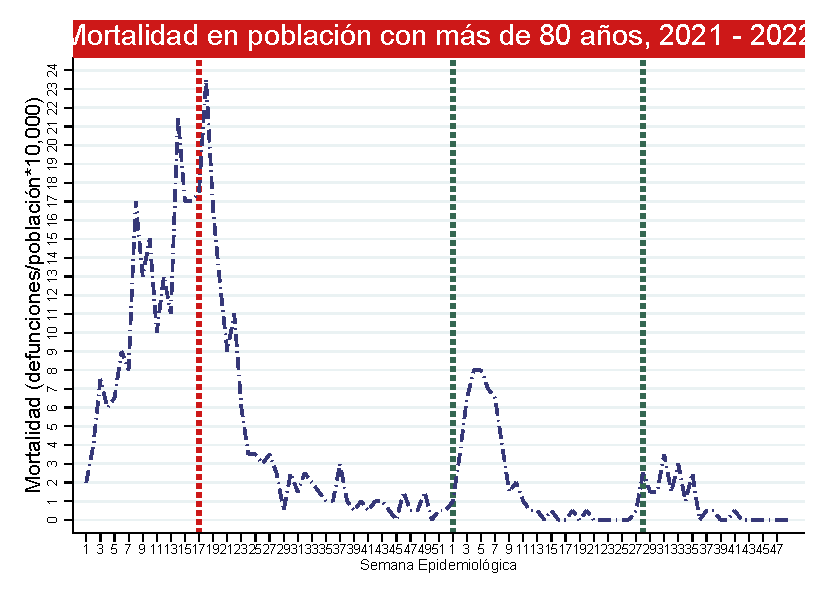
\includegraphics[width=\textwidth]{../figuras/mortalidad_edad_80.pdf}
		\caption{Más de 80 años}
		%\label{fig:}
	\end{subfigure}
	\hfill
	\begin{subfigure}[b]{0.45\textwidth}
		\centering
		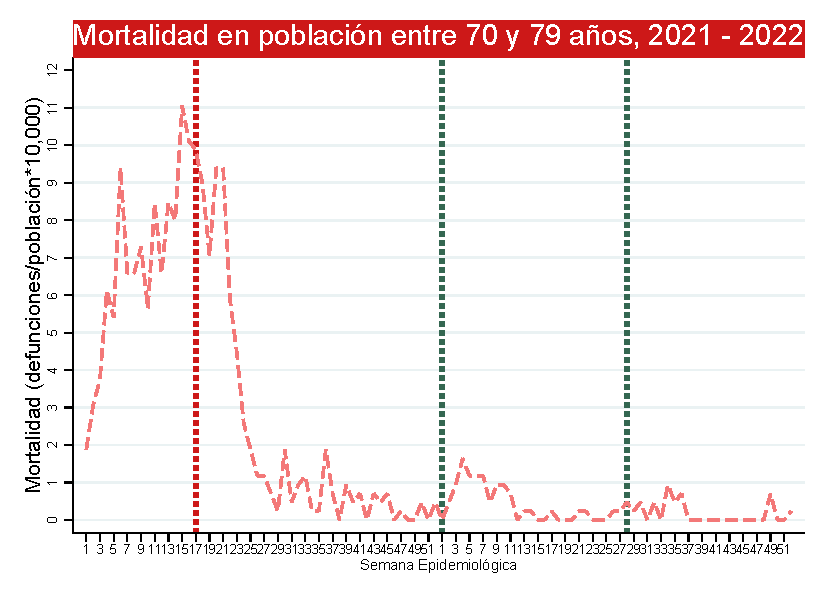
\includegraphics[width=\textwidth]{../figuras/mortalidad_edad_70.pdf}
		\caption{70 a 79 años}
		%\label{fig:70 a 79 años}
	\end{subfigure}

	\vspace{10mm}
	\begin{subfigure}[b]{0.45\textwidth}
		\centering
		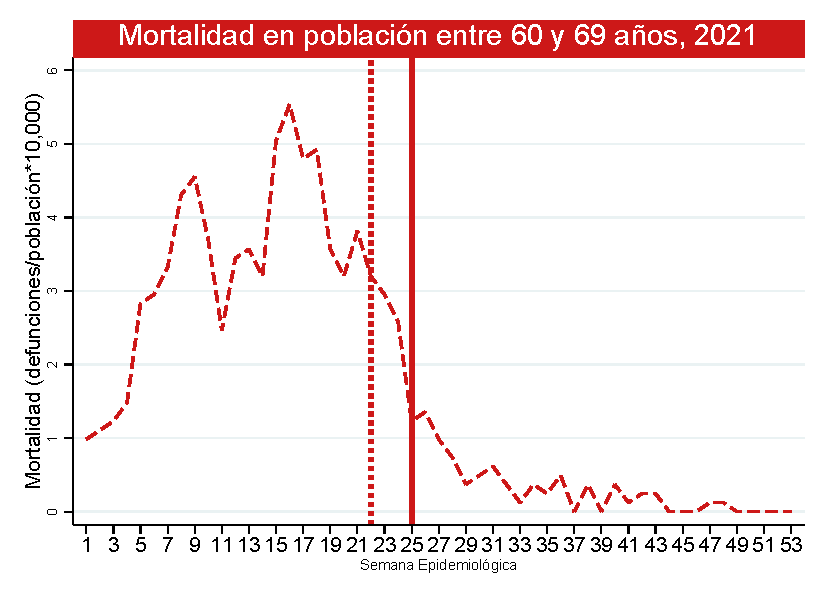
\includegraphics[width=\textwidth]{../figuras/mortalidad_edad_60.pdf}
		\caption{60 a 69 años}
		%\label{fig:60 a 69 años}
	\end{subfigure}
	\hfill
	\begin{subfigure}[b]{0.45\textwidth}
		\centering
		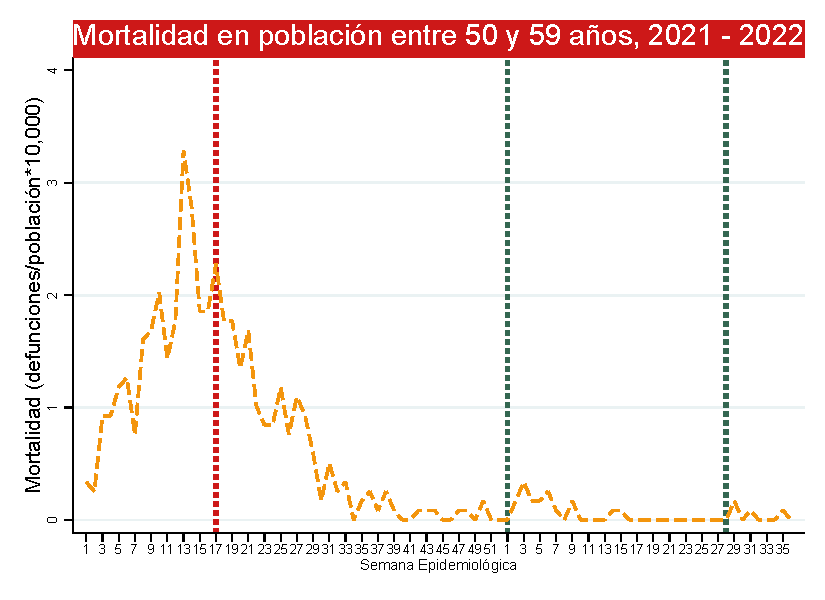
\includegraphics[width=\textwidth]{../figuras/mortalidad_edad_50.pdf}
		\caption{50 a 59 años}
		%\label{fig:50 a 59 años}
	\end{subfigure}

	\vspace{10mm}
	\begin{subfigure}[b]{0.45\textwidth}
		\centering
		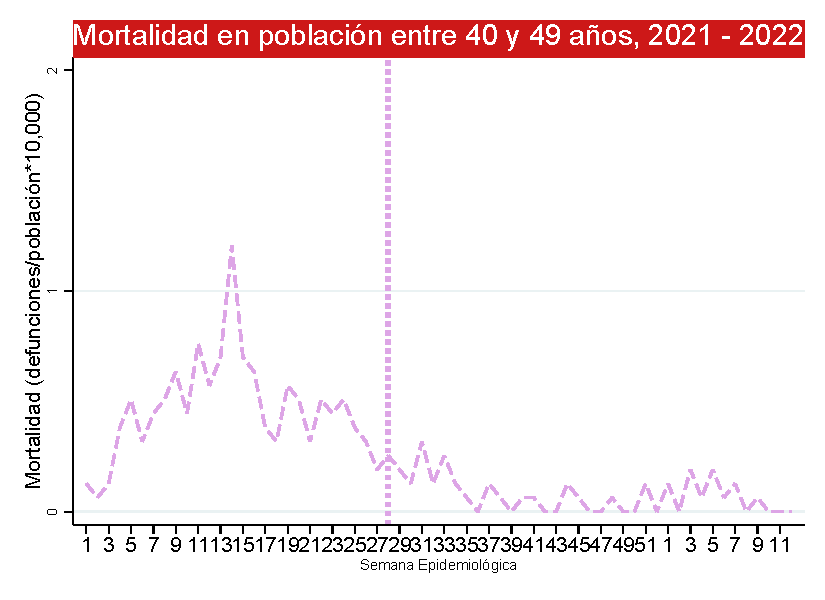
\includegraphics[width=\textwidth]{../figuras/mortalidad_edad_40.pdf}
		\caption{40 a 49 años}
		%\label{fig:40 a 49 años}
	\end{subfigure}
	\hfill
	\begin{subfigure}[b]{0.45\textwidth}
		\centering
		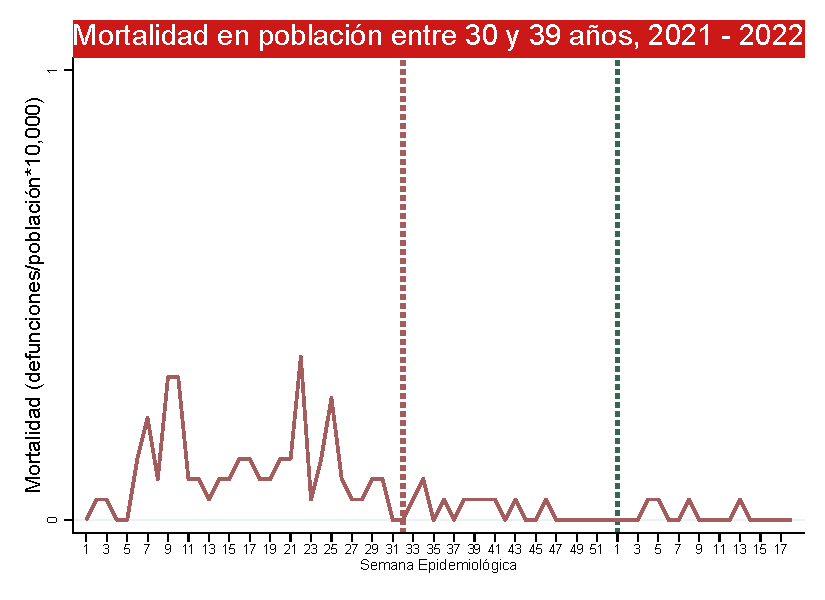
\includegraphics[width=\textwidth]{../figuras/mortalidad_edad_30.pdf}
		\caption{30 a 39 años}
		%\label{fig:40 a 49 años}
	\end{subfigure}
	\end{figure}

	\begin{figure}[h]
	\caption{Tasa de Mortalidad por COVID-19 por Grupo Etario hasta la SE 07-2022.}
	\label{fig:mortalidad_grupo_edad_2}
	\centering
	\begin{subfigure}[b]{0.45\textwidth}
		\centering
		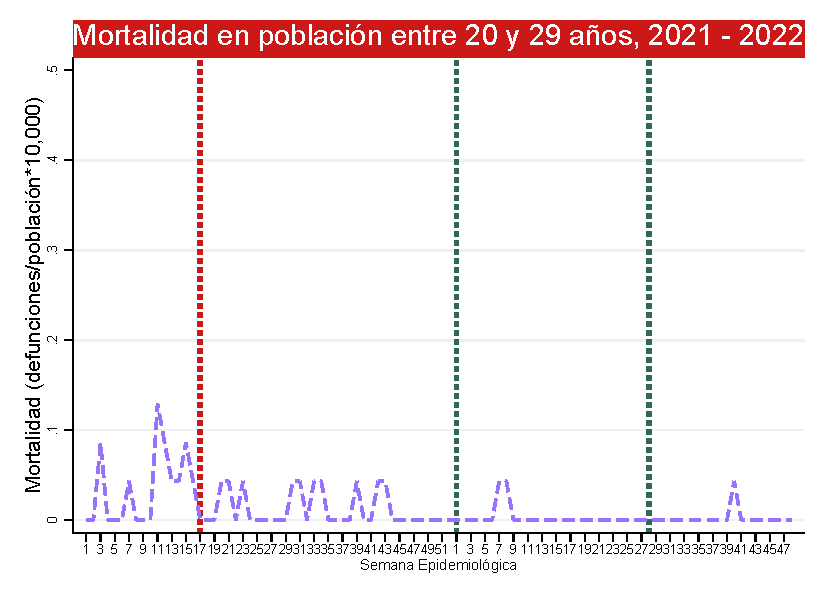
\includegraphics[width=\textwidth]{../figuras/mortalidad_edad_20.pdf}
		\caption{20 a 29 años}
		%\label{fig:40 a 49 años}
	\end{subfigure}

	\centering
	\begin{subfigure}[b]{0.45\textwidth}
		\centering
		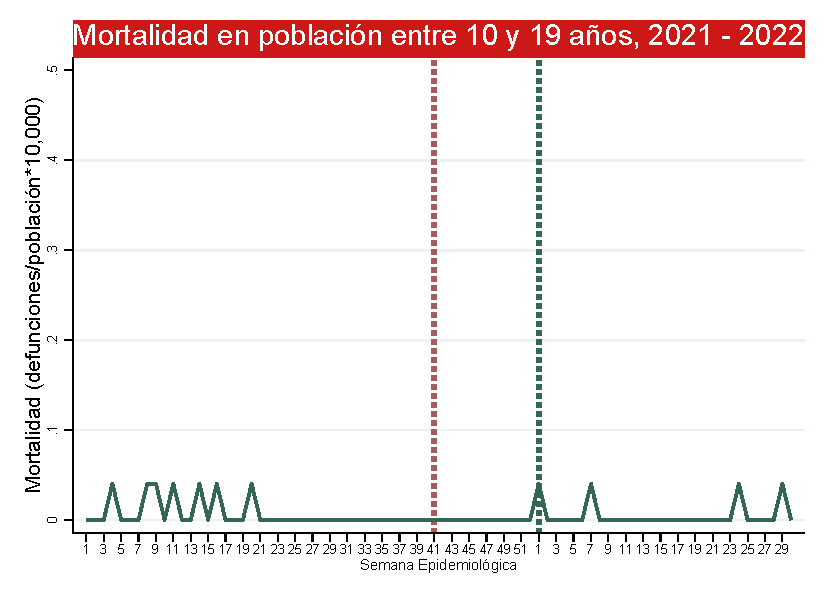
\includegraphics[width=\textwidth]{../figuras/mortalidad_edad_10.pdf}
		\caption{10 a 19 años}
		%\label{fig:40 a 49 años}
	\end{subfigure}
	
	\vspace{10mm}
	\begin{subfigure}[b]{0.45\textwidth}
		\centering
		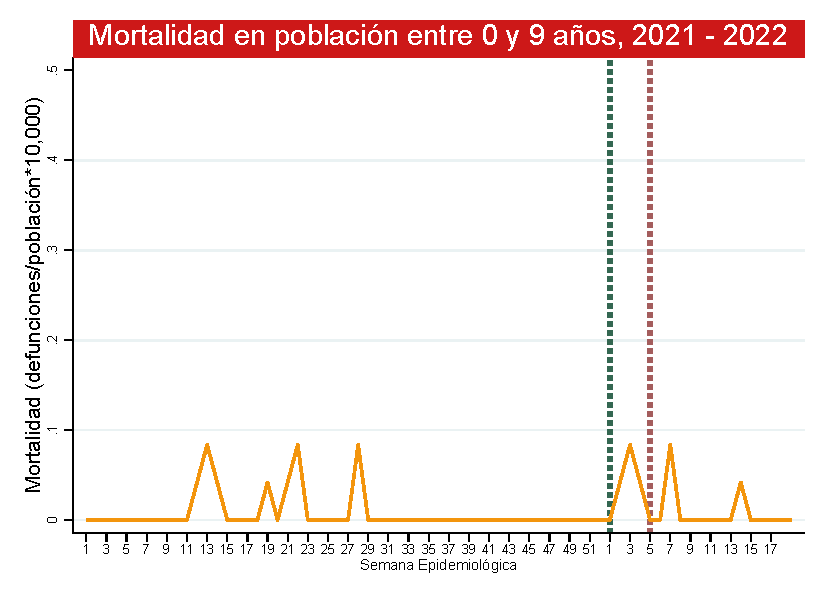
\includegraphics[width=\textwidth]{../figuras/mortalidad_edad_0.pdf}
		\caption{0 a 09 años}
		%\label{fig:40 a 49 años}
	\end{subfigure}
\end{figure}
\clearpage	
	\subsection*{Exceso de Muertes por Todas las Causas}
\noindent La Figura \ref{fig:exceso_regional} muestra la tendencia del exceso de muertes con respecto al año 2019. Para la SE 03 del 2022, hubo un exceso de defunciones de 25, sin embargo para la SE 04 se presentó un exceso negativo de -125 defunciones por todas las causas en comparación a la misma semana del año 2019.  

	\begin{figure}[h]
	\caption{Exceso de Fallecidos por Todas las Causas en la Región Cusco hasta la SE 07-2022.}\label{fig:exceso_regional}
	\begin{center}
		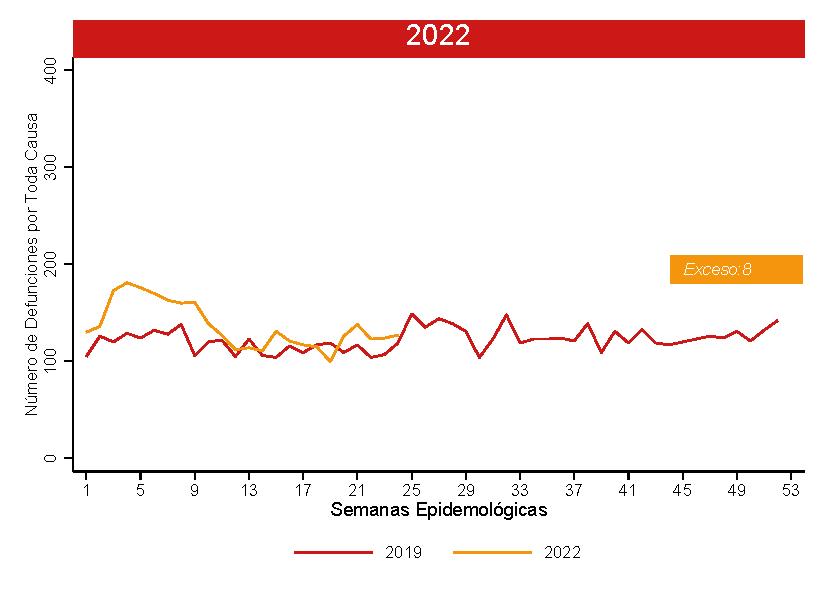
\includegraphics[width=0.85\linewidth]{../figuras/exceso_region_2022.pdf}
	\end{center}
	{\footnotesize {Fuente de datos: SISCOVID, NOTICOVID.}}
	\end{figure}
\clearpage

	\subsection*{Cobertura de Vacunación por COVID-19 en la Región Cusco, hasta la SE 07-2022.}
\noindent La Figura \ref{fig:vacuna_edad} muestra la cobertura de vacunación por grupo etario en la Región Cusco. El grupo etario con mejor cobertura es el de 70 a 79 años con 88,1 $\%$ de la población objetivo con 2 dosis aplicadas, seguido del grupo etario de 60 a 69 años con 87,6 $\%$. El grupo etario con menor cobertura es el de 12 a 19 años con el 61,4 $\%$ de cobertura.  

\begin{figure}[h]
	\caption{Cobertura de Vacunación por Grupo Etario en la Región Cusco hasta la SE 07-2022. }\label{fig:vacuna_edad}
	\begin{center}
		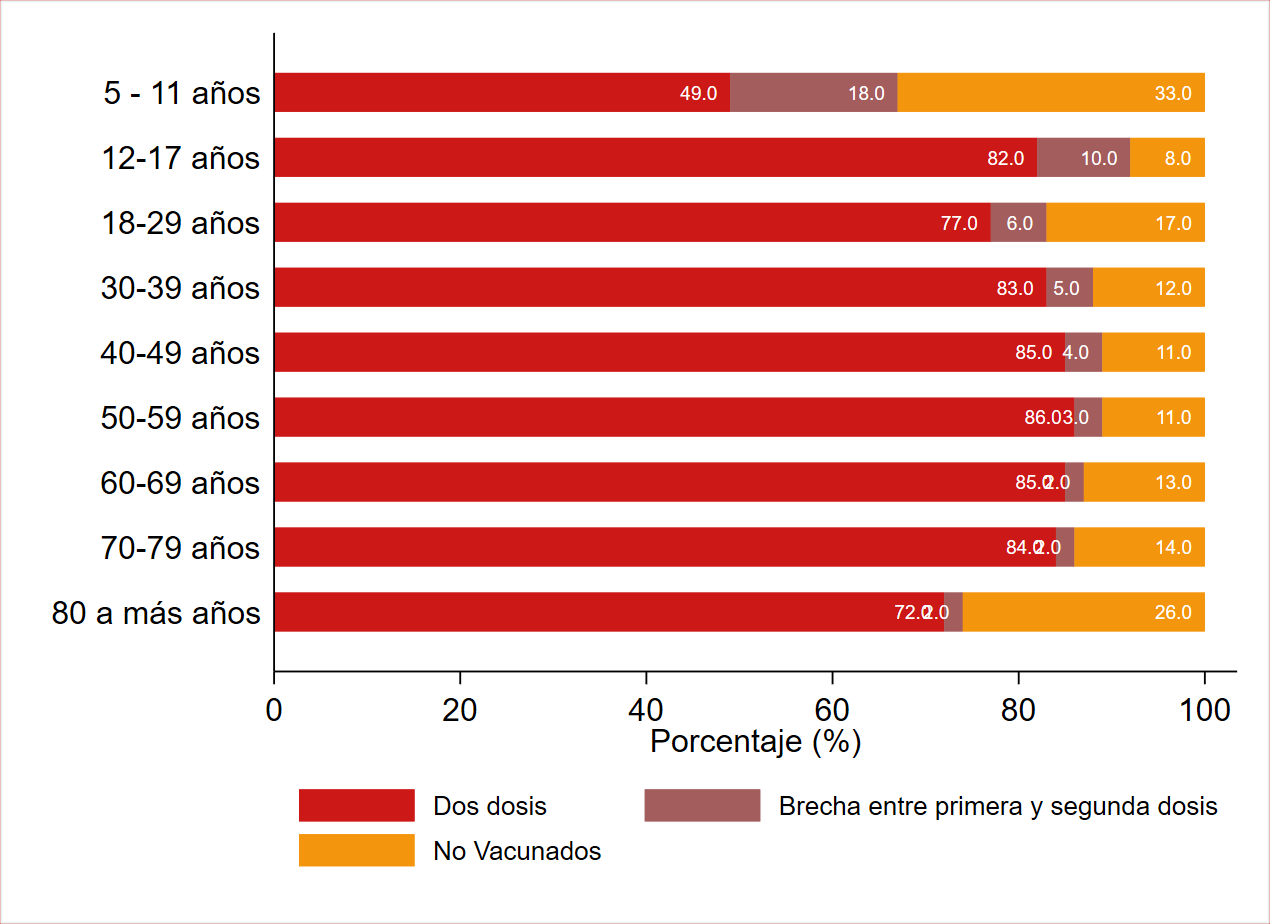
\includegraphics[width=0.90\linewidth]{../figuras/vacunacion_grupo_edad.png}
	\end{center}
	{\footnotesize {Fuente de datos: SICOVAC, HIS-MINSA.}}
\end{figure}

%La Figura \ref{fig:cobertura_vacunaci_provincia}  muestra la cobertura de vacunación en cada una de las provincias de Cusco por grupo etario. Es preciso señalar que la provincia de Espinar tiene la cobertura más baja de la región, en los grupos etarios desde los 50 años en adelante.
%
%\begin{figure}[h]
%	\caption{Cobertura de Vacunación por Provincia y por Grupo Etario en la Región Cusco, hasta la SE 51.}
%	\label{fig:cobertura_vacunaci_provincia}
%	\centering
%	\begin{subfigure}[b]{0.45\textwidth}
%		\centering
%		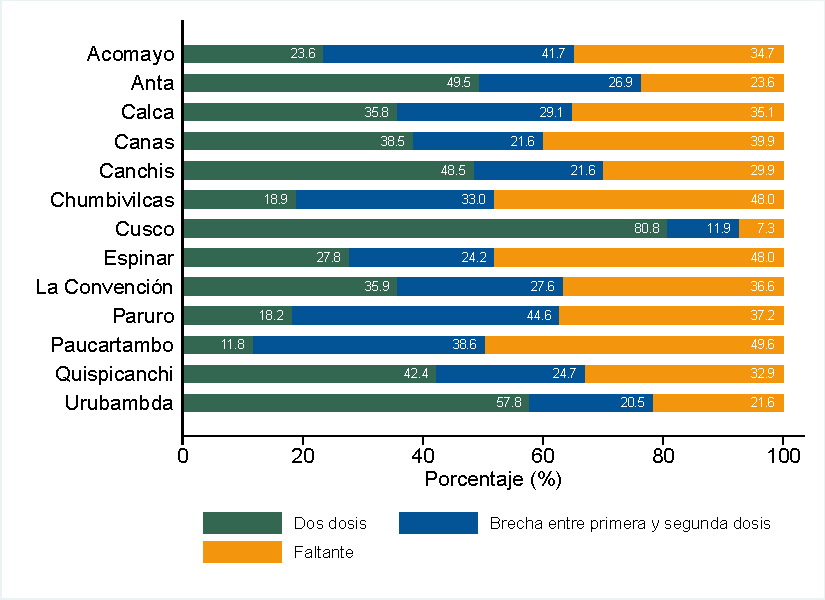
\includegraphics[width=\textwidth]{../figuras/vacunacion_provincial_edad_1}
%		\caption{ De 12 a 19 años}
%		%\label{fig:}
%	\end{subfigure}
%	\hfill
%	\begin{subfigure}[b]{0.45\textwidth}
%		\centering
%		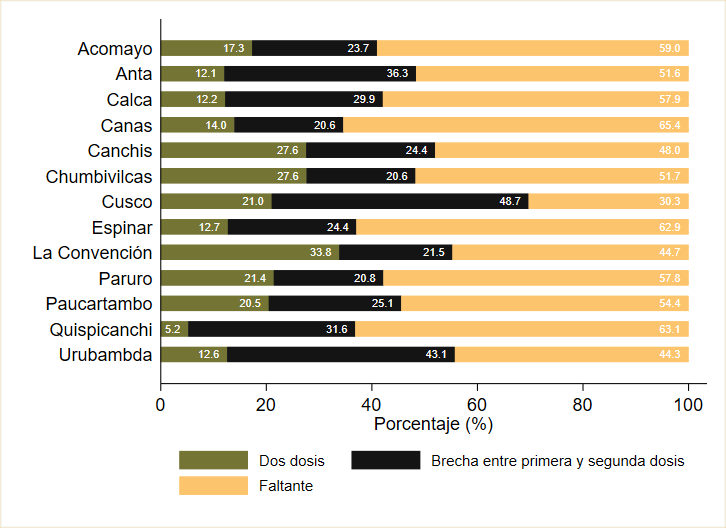
\includegraphics[width=\textwidth]{../figuras/vacunacion_provincial_edad_2}
%		\caption{De 20 a 29 años}
%		%\label{fig:70 a 79 años}
%	\end{subfigure}
%	\begin{subfigure}[b]{0.45\textwidth}
%		\centering
%		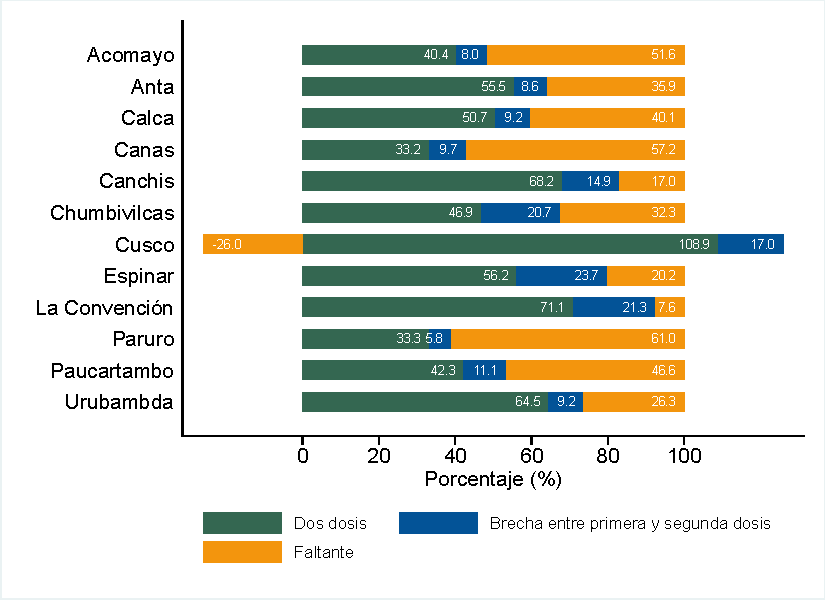
\includegraphics[width=\textwidth]{../figuras/vacunacion_provincial_edad_3}
%		\caption{De 30 a 39 años}
%		%\label{fig:60 a 69 años}
%	\end{subfigure}
%	\hfill
%	\begin{subfigure}[b]{0.45\textwidth}
%		\centering
%		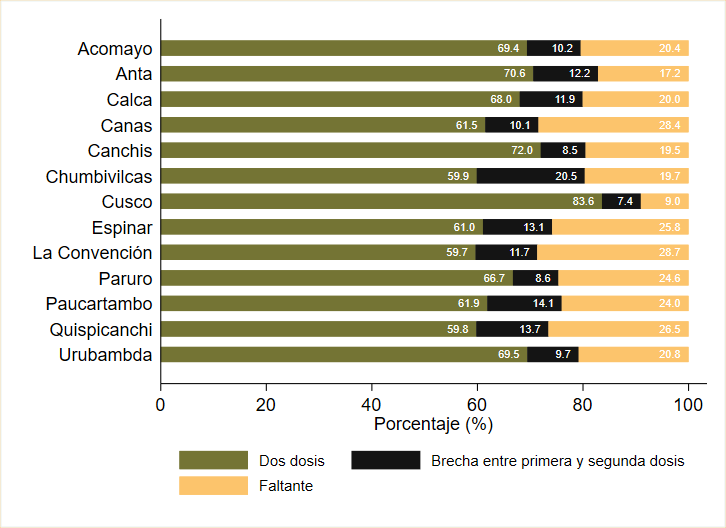
\includegraphics[width=\textwidth]{../figuras/vacunacion_provincial_edad_4}
%		\caption{De 40 a 49 años}
%		%\label{fig:50 a 59 años}
%	\end{subfigure}
%	\begin{subfigure}[b]{0.45\textwidth}
%		\centering
%		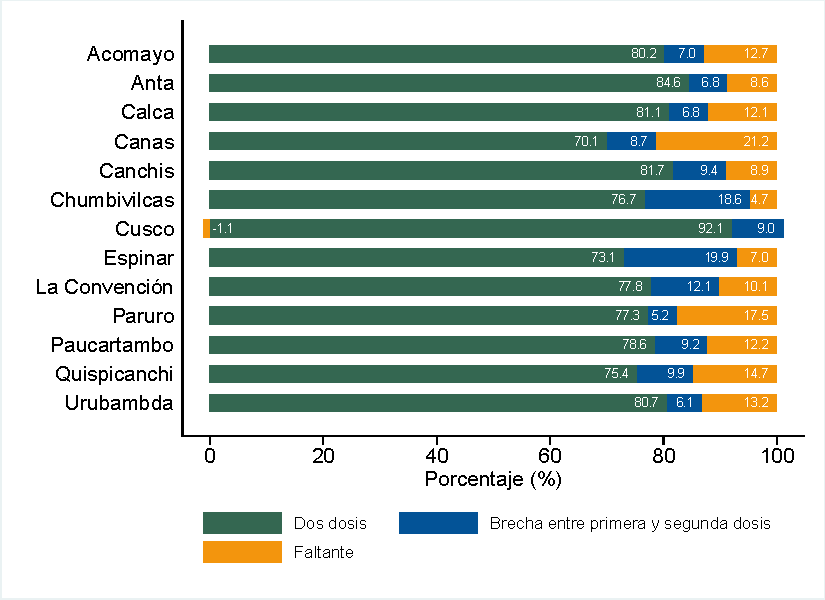
\includegraphics[width=\textwidth]{../figuras/vacunacion_provincial_edad_5}
%		\caption{De 50 a 59 años}
%		%\label{fig:40 a 49 años}
%	\end{subfigure}
%	\hfill
%	\begin{subfigure}[b]{0.45\textwidth}
%		\centering
%		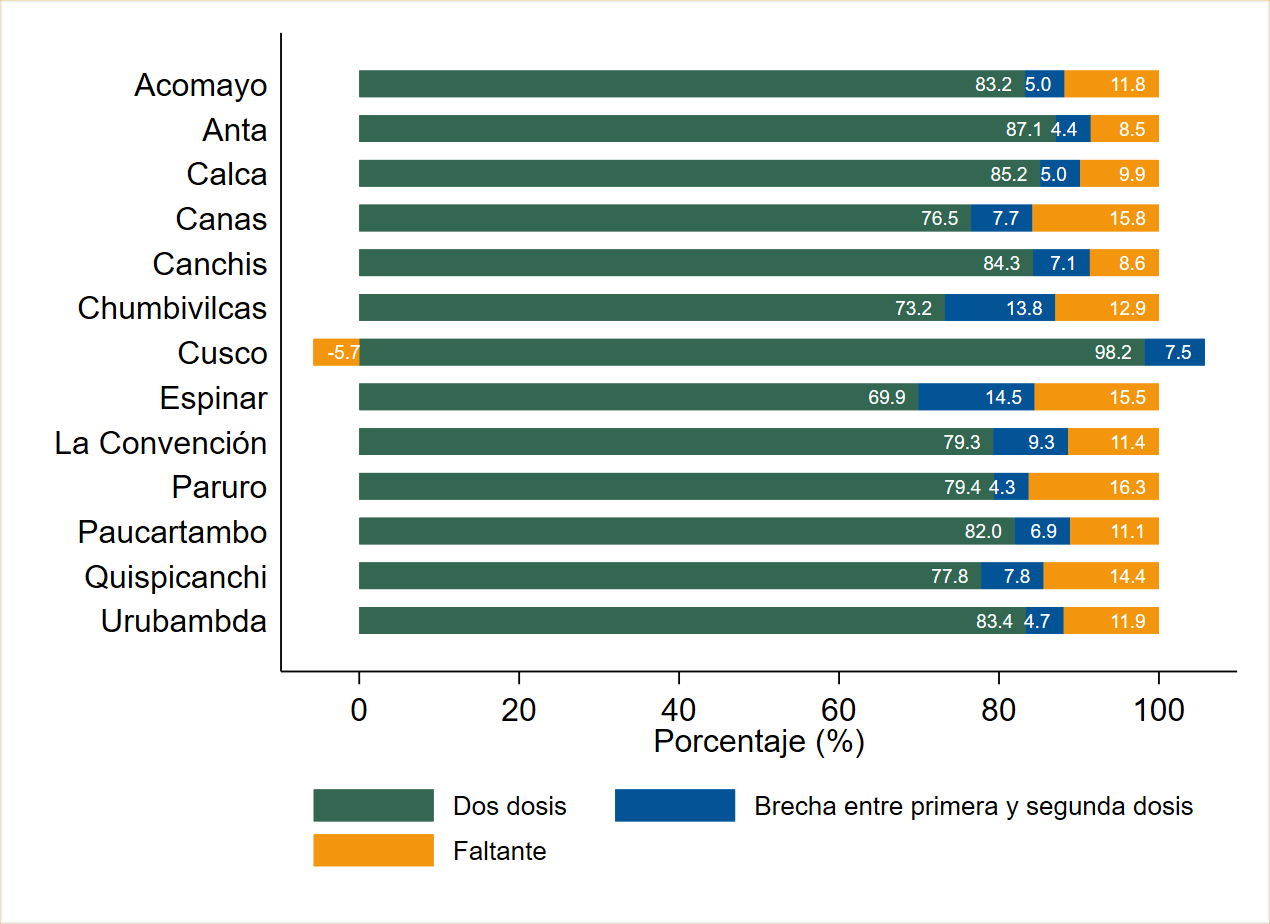
\includegraphics[width=\textwidth]{../figuras/vacunacion_provincial_edad_6}
%		\caption{De 60 a 69 años}
%		%\label{fig:40 a 49 años}
%	\end{subfigure}
%\begin{subfigure}[b]{0.45\textwidth}
%	\centering
%	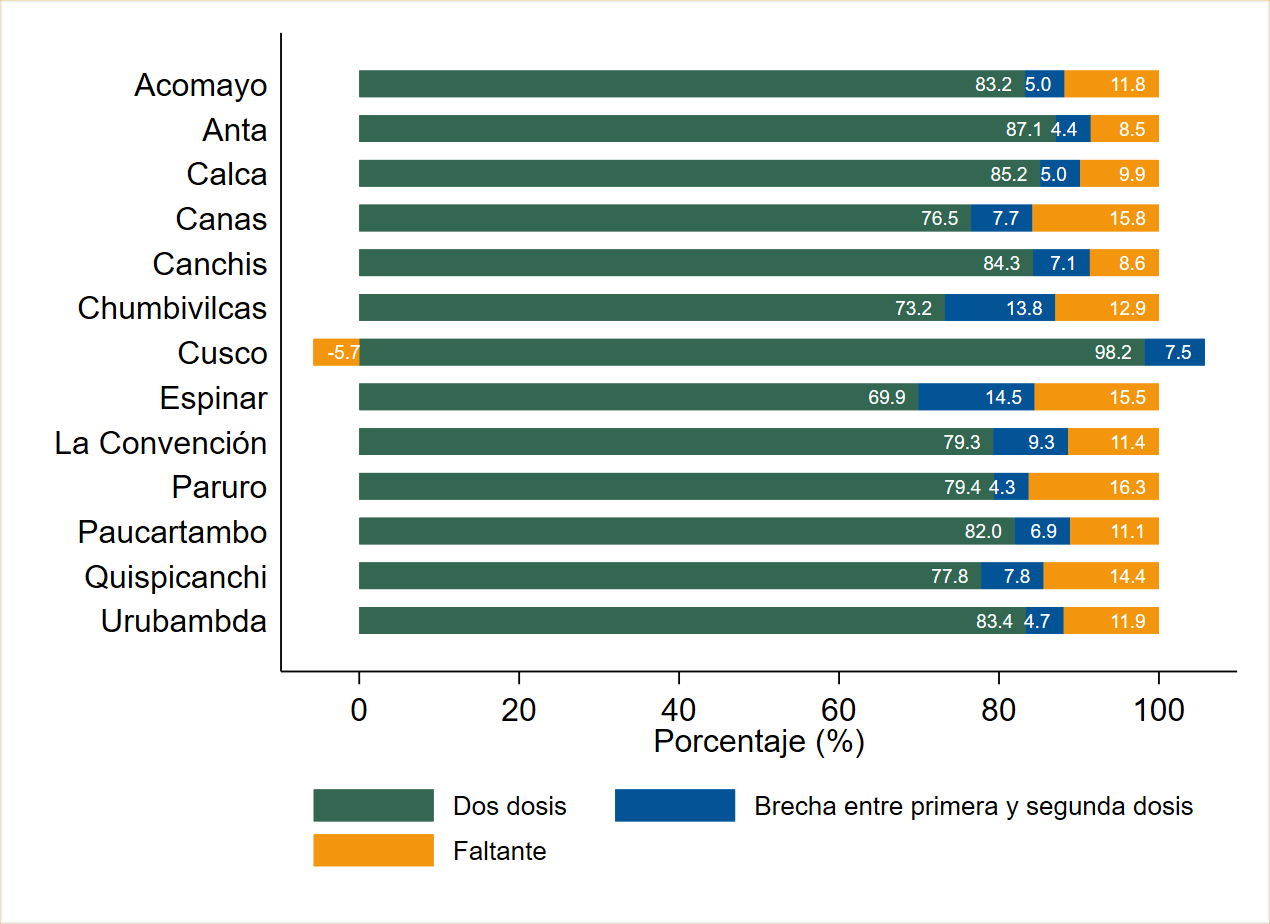
\includegraphics[width=\textwidth]{../figuras/vacunacion_provincial_edad_6}
%	\caption{De 70 a 79 años}
%	%\label{fig:40 a 49 años}
%\end{subfigure}
%\hfill
%\begin{subfigure}[b]{0.45\textwidth}
%	\centering
%	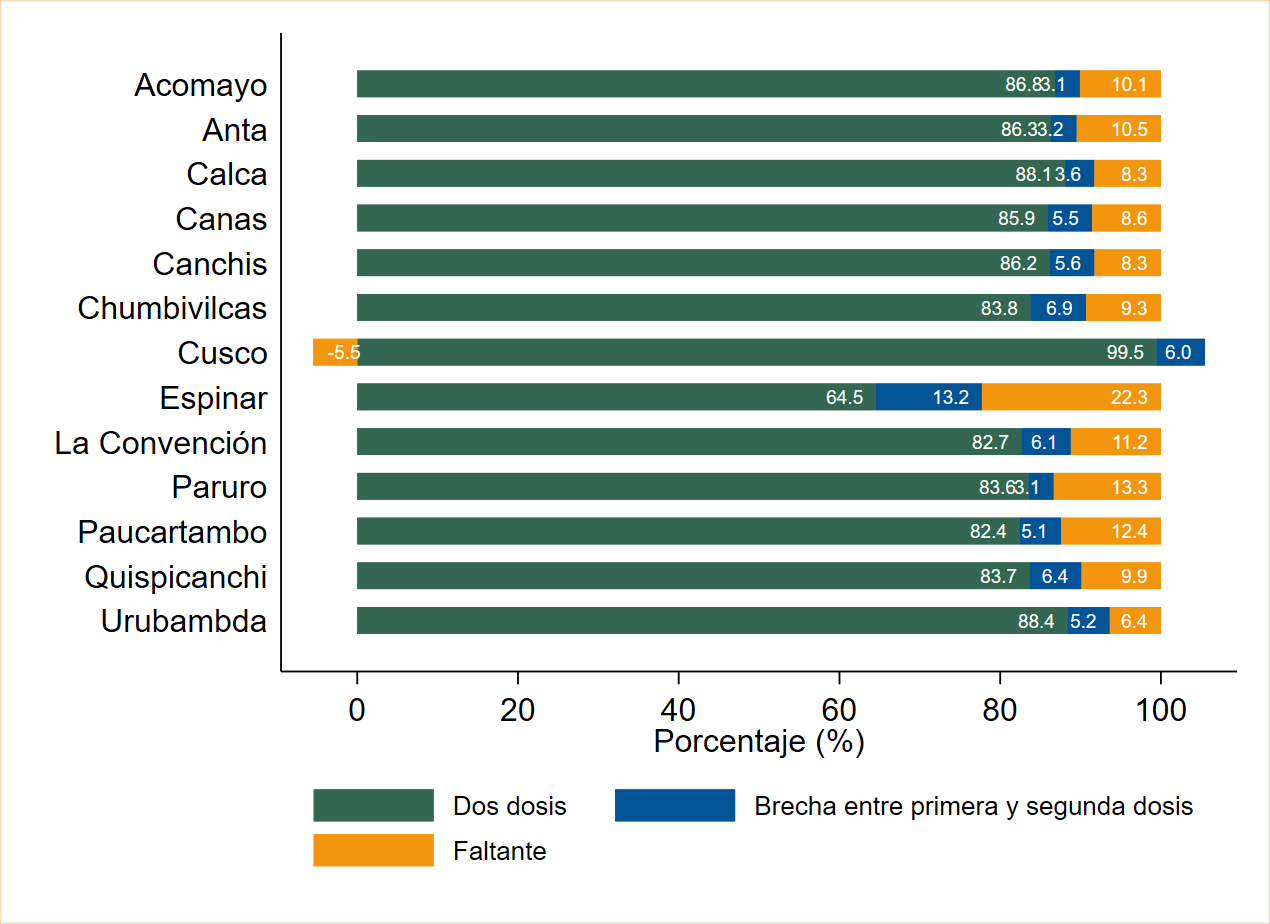
\includegraphics[width=\textwidth]{../figuras/vacunacion_provincial_edad_7}
%	\caption{Más de 80 años}
%	%\label{fig:40 a 49 años}
%\end{subfigure}
%\end{figure}

\clearpage
\subsection*{Ocupación de Camas}
\noindent La disponibilidad y ocupación de camas UCI se ve resumida en la Figura \ref{fig:ocupacion_uci}, se evidencia que desde la primera semana del 2022, el porcentaje de ocupación muestra un pendiente en ascenso. Para la SE 03 se aprecia un incremento del 29$\%$ con respecto al porcentaje de ocupación de la última semana del 2021, llegando a tener solo 19$\%$ de camas UCI disponibles en la SE 03.    

\begin{figure}[h]
	\caption{Ocupación de Camas UCI COVID-19 en la Región Cusco hasta la SE 07- 2022.}\label{fig:ocupacion_uci}
	\begin{center}
		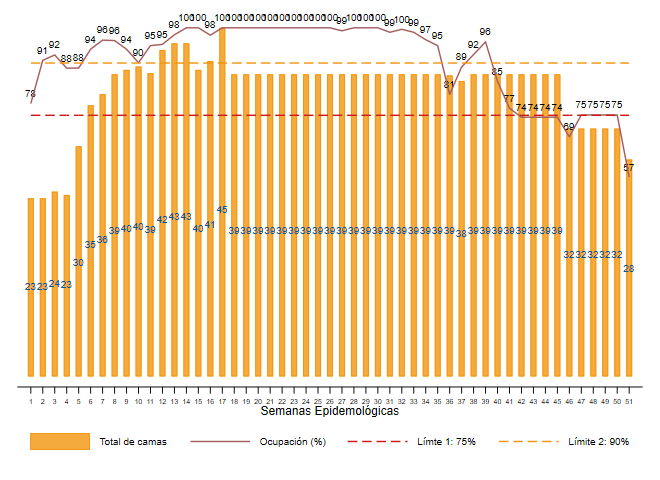
\includegraphics[width=0.95\linewidth]{../figuras/uci.png}
	\end{center}
	{\footnotesize {Fuente de datos: REFERENCIAS Y CONTRAREFERENCIAS.}}
\end{figure}
\cleardoublepage

En la Figura \ref{fig:ocupacion_3_nivel}, se plasma el porcentaje de ocupación y número de camas no-UCI COVID-19 en el nivel Hospitalario III. Al igual que las camas UCI, el porcentaje de ocupación de camas no UCI COVID-19 presenta una pendiente en ascenso desde la primera semana del 2022, llegando a ser del  47$\%$ en la SE 03. Cabe resaltar que el porcentaje de ocupación aún no iguala al porcentaje de ocupación más alto de la segunda ola.  
  
\begin{figure}[htpb]
	\caption{Ocupación de Camas no UCI COVID-19 en el nivel III en la Región Cusco hasta la SE 07-2022.}\label{fig:ocupacion_3_nivel}
	\begin{center}
		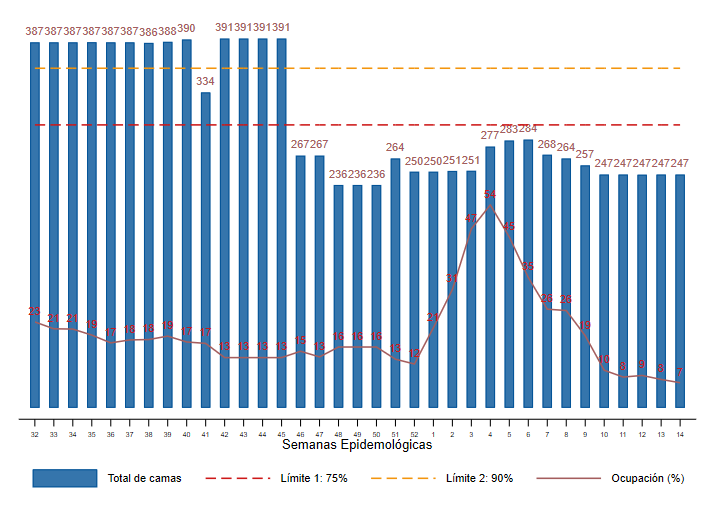
\includegraphics[width=0.95\linewidth]{../figuras/nivel_3.png}
	\end{center}
	{\footnotesize {Fuente de datos: REFERENCIAS Y CONTRAREFERENCIAS.}}
\end{figure}

\clearpage

En la Figura \ref{fig:ocupacion_2nivel}, se observa el número de camas disponibles y su porcentaje de ocupación en el Nivel II. Este porcentaje muestra un pendiente en ascenso desde la primera semana del 2022, sin embargo el porcentaje de ocupación aún es bajo, teniendo un 83$\%$ de camas disponibles para la SE 03.   

\begin{figure}[h]
	\caption{Disponibilidad y Ocupación de Camas-COVID a Nivel de Hospitales del Nivel II en la Región Cusco hasta la SE 07-2022.}\label{fig:ocupacion_2nivel}
	\begin{center}
		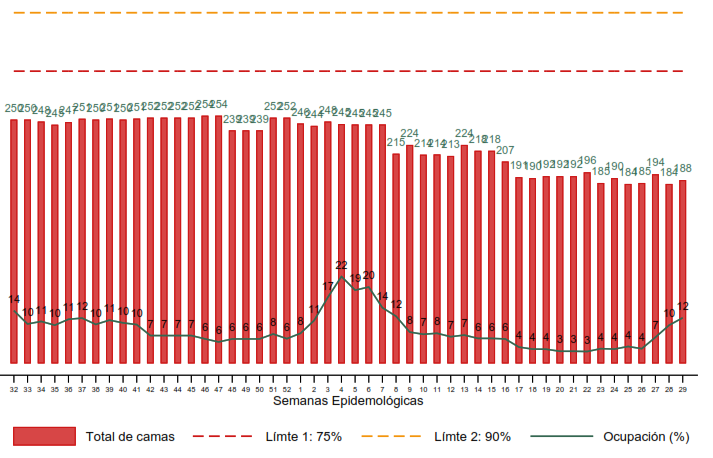
\includegraphics[width=0.95\linewidth]{../figuras/nivel_2.png}
	\end{center}
	{\footnotesize {Fuente de datos: REFERENCIAS Y CONTRAREFERENCIAS.}}
\end{figure}
\clearpage
\begin{landscape}
	
	\subsection*{Evaluación Provincial de la Infección por COVID-19 para el año 2022.} 
	
	\begin{tabular}{@{}lrrrrr@{}}
	\rowcolor[HTML]{ECF4FF} 
	\textbf{Provincias}                   & \multicolumn{1}{l}{\cellcolor[HTML]{ECF4FF}\textbf{población}} & \multicolumn{1}{l}{\cellcolor[HTML]{ECF4FF}\textbf{Pruebas Totales}} & \multicolumn{1}{l}{\cellcolor[HTML]{ECF4FF}\textbf{Funciones}} & \multicolumn{1}{l}{\cellcolor[HTML]{ECF4FF}\textbf{Tasa de letalidad}} & \multicolumn{1}{l}{\cellcolor[HTML]{ECF4FF}\textbf{\begin{tabular}[c]{@{}l@{}}tasa de mortalidad x \\   100.000 hab\end{tabular}}} \\
	\cellcolor[HTML]{FD6864}CANCHIS       & 105,049                                                        & 1,545                                                                & 5                                                              & 0.3\%                                                                  & 4.8                                                                                                                                \\
	\cellcolor[HTML]{FD6864}PAUCARTAMBO   & 52,989                                                         & 301                                                                  & 2                                                              & 0.7\%                                                                  & 3.8                                                                                                                                \\
	\cellcolor[HTML]{FD6864}LA CONVENCION & 185,793                                                        & 2,623                                                                & 7                                                              & 0.3\%                                                                  & 3.8                                                                                                                                \\
	\cellcolor[HTML]{FFFC9E}CUSCO         & 463,656                                                        & 16,911                                                               & 9                                                              & 0.1\%                                                                  & 1.9                                                                                                                                \\
	\cellcolor[HTML]{FFFC9E}ESPINAR       & 71,304                                                         & 479                                                                  & 1                                                              & 0.2\%                                                                  & 1.4                                                                                                                                \\
	\cellcolor[HTML]{FFFC9E}CALCA         & 76,462                                                         & 462                                                                  & 1                                                              & 0.2\%                                                                  & 1.3                                                                                                                                \\
	\cellcolor[HTML]{9AFF99}CHUMBIVILCAS  & 84,925                                                         & 448                                                                  & 1                                                              & 0.2\%                                                                  & 1.2                                                                                                                                \\
	\cellcolor[HTML]{9AFF99}QUISPICANCHI  & 92,566                                                         & 735                                                                  & 1                                                              & 0.1\%                                                                  & 1.1                                                                                                                                \\
	\cellcolor[HTML]{9AFF99}ACOMAYO       & 28,477                                                         & 149                                                                  & 0                                                              & 0.0\%                                                                  & 0.0                                                                                                                                \\
	\cellcolor[HTML]{9AFF99}ANTA          & 57,731                                                         & 480                                                                  & 0                                                              & 0.0\%                                                                  & 0.0                                                                                                                                \\
	\cellcolor[HTML]{9AFF99}CANÁS         & 40,420                                                         & 206                                                                  & 0                                                              & 0.0\%                                                                  & 0.0                                                                                                                                \\
	\cellcolor[HTML]{9AFF99}PARURO        & 31,264                                                         & 132                                                                  & 0                                                              & 0.0\%                                                                  & 0.0                                                                                                                                \\
	\cellcolor[HTML]{9AFF99}URUBAMBÁ      & 66,439                                                         & 900                                                                  & 0                                                              & 0.0\%                                                                  & 0.0                                                                                                                                \\
	& \multicolumn{1}{l}{}                                           & \multicolumn{1}{l}{}                                                 & \multicolumn{1}{l}{}                                           & \multicolumn{1}{l}{}                                                   & \multicolumn{1}{l}{}                                                                                                               \\
	\rowcolor[HTML]{ECF4FF} 
	\textbf{Totales generales}            & \textbf{1,357,075}                                             & \textbf{25,371}                                                      & \textbf{27}                                                    & \textbf{0.11\%}                                                        & \textbf{2.0}                                                                                                                      
\end{tabular}
	
	
	{\footnotesize Fuente de datos: NOTICOVID, SISCOVID, SINADEF. Actualizado a la SE 07-2022.}
	
	\noindent 
	
\end{landscape}
%---------------------------------------------------------------------------
% CAPÍTULO: EVALUACIÓN DE PROVINCIAS
%---------------------------------------------------------------------------

%insertar el cover del capitulo
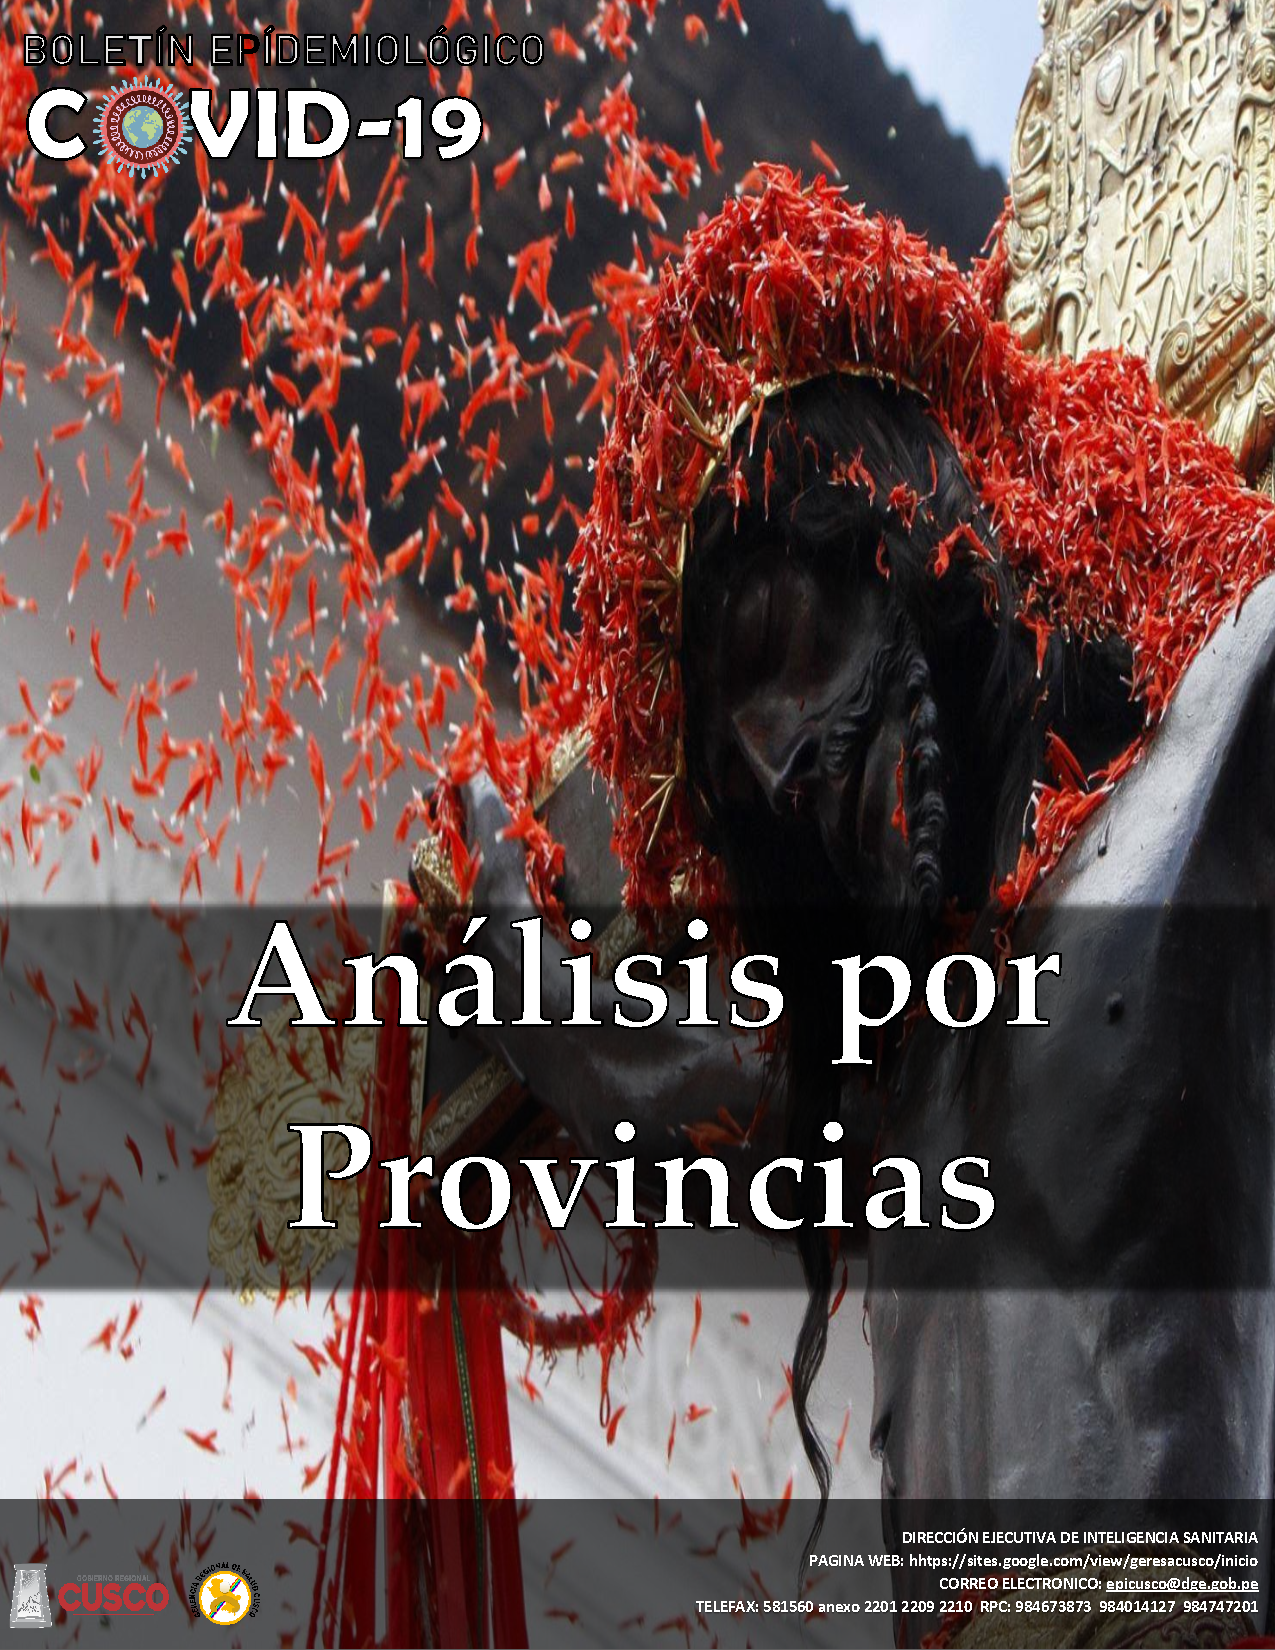
\includepdf[pages={1}]{../editorial/5.pdf}
\clearpage

	\section*{Evaluación para Provincias Priorizadas}
\addcontentsline{toc}{chapter}{Evaluación para Provincias Priorizadas}
\noindent La Figura \ref{fig:incidencia_provincias} muestra las tasas de incidencia acumulada por provincia desde el 1 de enero hasta el 27 de enero del 2022, ordenadas de mayor a menor, se evidencia que la mayor tasa de incidencia acumulada es la provincia de Cusco (388,7 casos / 10 000 personas), seguida de la provincia de Canchis (171,6 casos/ 10 000 personas)  y La Convención (151,6 casos/ 10 000 personas).

\begin{figure}[!htpb]
	\caption{Tasa de Incidencia Acumulada por Provincia en la Región Cusco, hasta el 22 de febrero del 2022*. }\label{fig:incidencia_provincias}
	\begin{center}
		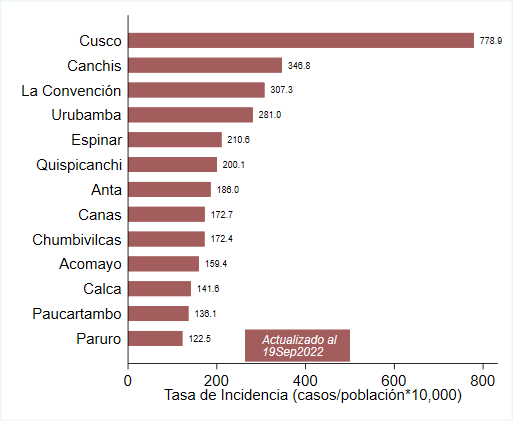
\includegraphics[width=0.75\linewidth]{../figuras/incidencia_provincial_2022.png}
	\end{center}
	{\footnotesize {
	Fuente de datos: SISCOVID, NOTICOVID.(*)Se considera como caso positivo sólo a pacientes con prueba molecular o antigénica positiva}}
\end{figure}


La Figura \ref{fig:mortalidad_ordenada} muestra a las provincias de la región ordenadas de mayor a menor según la tasa de mortalidad acumulada, desde el 1 de enero hasta el 27 de enero del 2022. La mayor tasa de mortalidad persiste en la provincia de Canchis con 0,9 defunciones / 10 000 personas.   

\begin{figure}[h]
	\caption{Tasa de Mortalidad Acumulada por Provincia en la Región Cusco, hasta la SE 07-2022. }\label{fig:mortalidad_ordenada}
	\begin{center}
		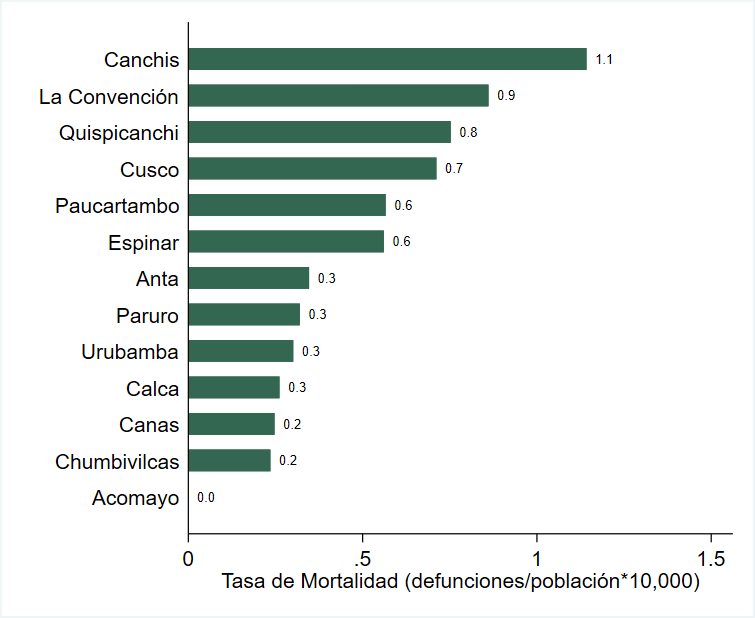
\includegraphics[width=0.65\linewidth]{../figuras/mortalidad_provincial_2022.png}
	\end{center}
	{\footnotesize {Fuente de datos: SISCOVID, NOTICOVID.}}
\end{figure}

La Figura \ref{fig:incidencia_provincial} muestra la tendencia de la incidencia acumulada a través del año 2022. Se observa que en todas las provincias la tendencia de la incidencia muestra un marcado crecimiento. 
%
\begin{figure}[h]
	\caption{Tendencia Provincial de Incidencia acumulada de COVID-19 hasta la SE 07-2022. }\label{fig:incidencia_provincial}
	\begin{center}
		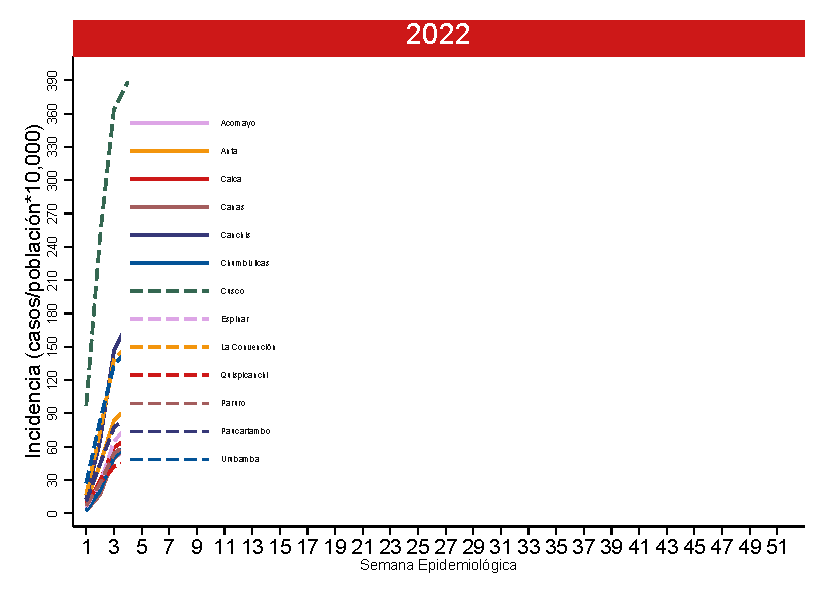
\includegraphics[width=0.65\linewidth]{../figuras/incidencia_provincial_2022.pdf}
	\end{center}
	{\footnotesize {Fuente de datos: SINADEF.}}
\end{figure}

\clearpage
	
\section*{Evaluación Provincial de 5 Indicadores}
		\noindent El objetivo de estas figuras es comparar a cada provincia consigo misma de acuerdo a su historia  en la primera ola (en el año 2020). Se evaluaron los siguientes indicadores: incidencia (tomando en cuenta pruebas moleculares y antigénicas), tasa de mortalidad, tasa de positividad por prueba molecular, tasa de positividad por prueba antigénica, y exceso de defunciones para cada provincia.
		
		\subsection*{Provincia de Acomayo}
		\noindent La Figura \ref{fig:inc_mort_acomayo} se evidencia un ascenso sostenido de la tasa de incidencia a partir de la SE 01 del año 2022, mientras que la tasa de mortalidad se ha mantenido constante. 
		\noindent La figura Figura \ref{fig:positividad_acomayo} muestra un ascenso de las tasas de positividad de tanto pruebas antigénicas como moleculares desde la misma fecha que la tasa de incidencia. 
		
		 En la Figura \ref{fig:exceso_acomayo} se muestra que hay un exceso negativo de menos 6 defunciones respecto al año 2019.
		
		\begin{figure}[h]
			\caption{Tasa de Incidencia y Mortalidad Comparativa en la Provincia de Acomayo hasta la SE 07-2022.}\label{fig:inc_mort_acomayo}
			\begin{center}
				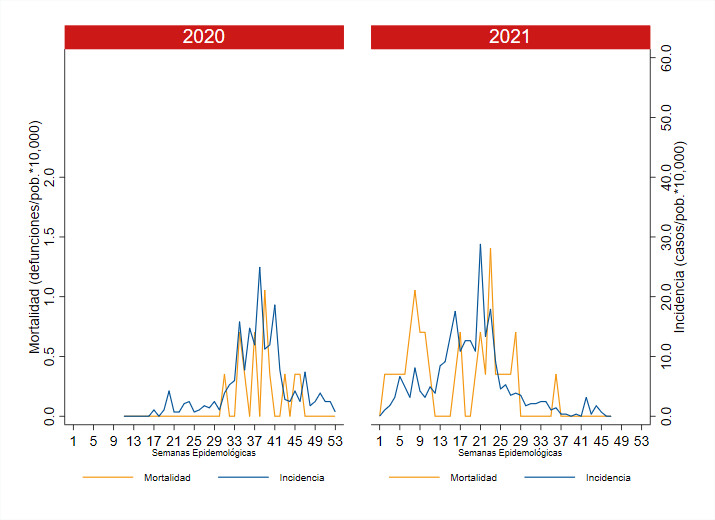
\includegraphics[width=0.65\linewidth]{../figuras/incidencia_mortalidad_20_21_1.png}
			\end{center}
			{\footnotesize {Fuente de datos: NOTICOVID, SISCOVID, SINADEF.}}
		\end{figure}
		
		\begin{figure}[h]
			\caption{Tasa de Positividad de Prueba Molecular y Antigénica Comparativa en la Provincia de Acomayo hasta la SE 07-2022. }\label{fig:positividad_acomayo}
			\begin{center}
				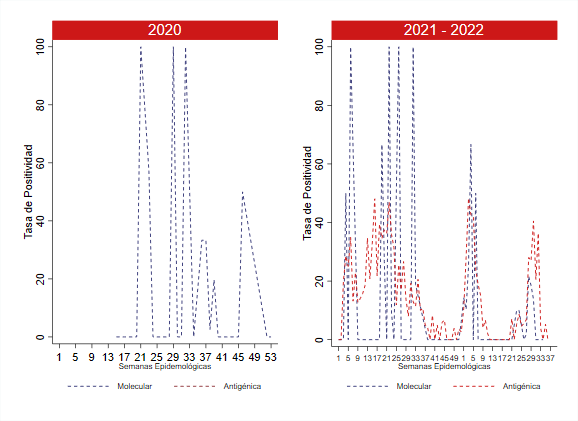
\includegraphics[width=0.7\linewidth]{../figuras/positividad_20_21_1.png}
			\end{center}
			{\footnotesize {Fuente de datos: NOTICOVID, SISCOVID.}}
		\end{figure}
		
		\begin{figure}[h]
			\caption{Exceso de Defunciones Comparativo en la Provincia de Acomayo hasta la SE 07-2022.}\label{fig:exceso_acomayo}
			\begin{center}
				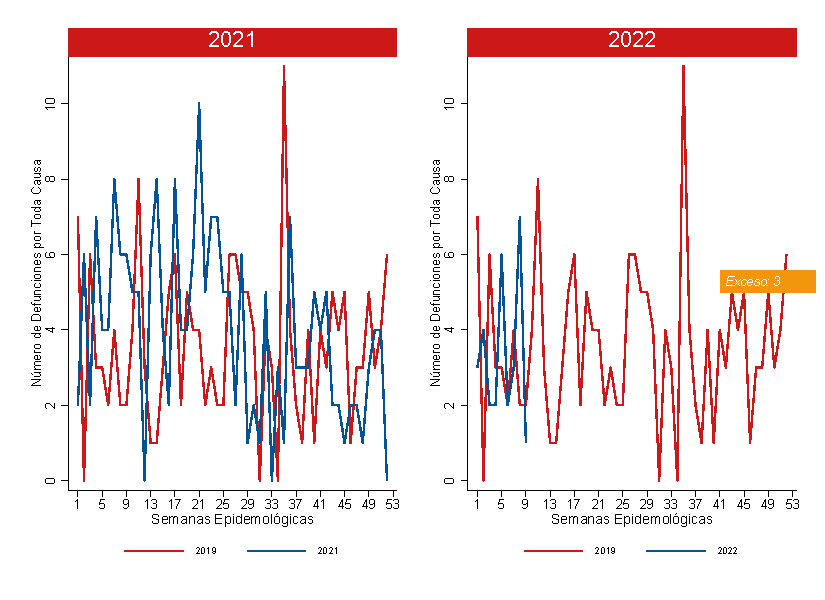
\includegraphics[width=0.7\linewidth]{../figuras/exceso_1.pdf}
			\end{center}
			{\footnotesize {Fuente de datos: SINADEF.}}
		\end{figure}
		
		% Anta
		\clearpage
		
		\subsection*{Provincia de Anta}
		\noindent La Figura \ref{fig:inc_mort_anta}  se evidencia un ascenso sostenido de la tasa de incidencia a partir de la SE 01 del año 2022, mientras que la tasa de mortalidad se ha mantenido constante con cero defunciones. 
		\noindent La Figura
		\ref{fig:positividad_anta} muestra el ascenso de las tasas de positividad de ambas pruebas desde la misma fecha que la tasa de incidencia.. 
		
		En la Figura \ref{fig:exceso_anta} se muestra que hay un exceso negativo de menos 11 defunciones respecto al año 2019.
		
		\begin{figure}[h]
			\caption{Tasa de Incidencia y Mortalidad Comparativa en la Provincia de Anta hasta la SE 07-2022.}\label{fig:inc_mort_anta}
			\begin{center}
				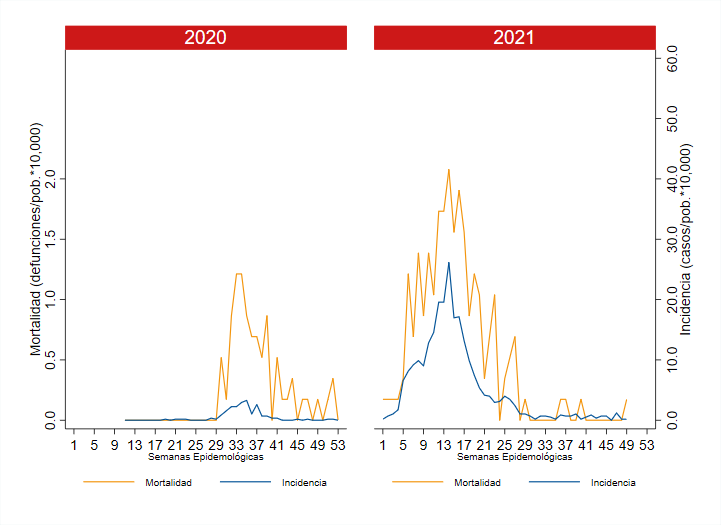
\includegraphics[width=0.7\linewidth]{../figuras/incidencia_mortalidad_20_21_2.png}
			\end{center}
			{\footnotesize {Fuente de datos: NOTICOVID, SISCOVID, SINADEF.}}
		\end{figure}
		
		\begin{figure}[h]
			\caption{Tasa de Positividad de Prueba Molecular y Antigénica Comparativa en la Provincia de Anta hasta la SE 07-2022.}\label{fig:positividad_anta}
			\begin{center}
				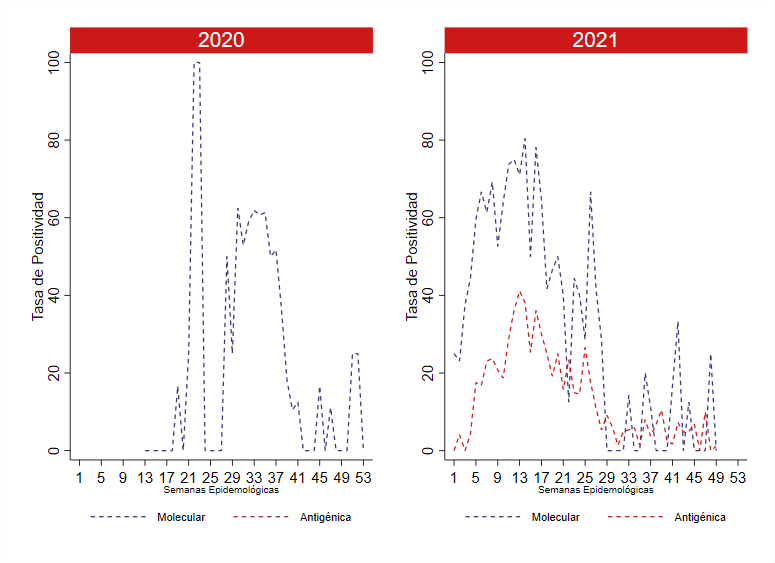
\includegraphics[width=0.7\linewidth]{../figuras/positividad_20_21_2.png}
			\end{center}
			{\footnotesize {Fuente de datos: NOTICOVID, SISCOVID.}}
		\end{figure}
		
		\begin{figure}[h]
			\caption{Exceso de Defunciones Comparativo en la Provincia de Anta hasta la SE 07-2022.}\label{fig:exceso_anta}
			\begin{center}
				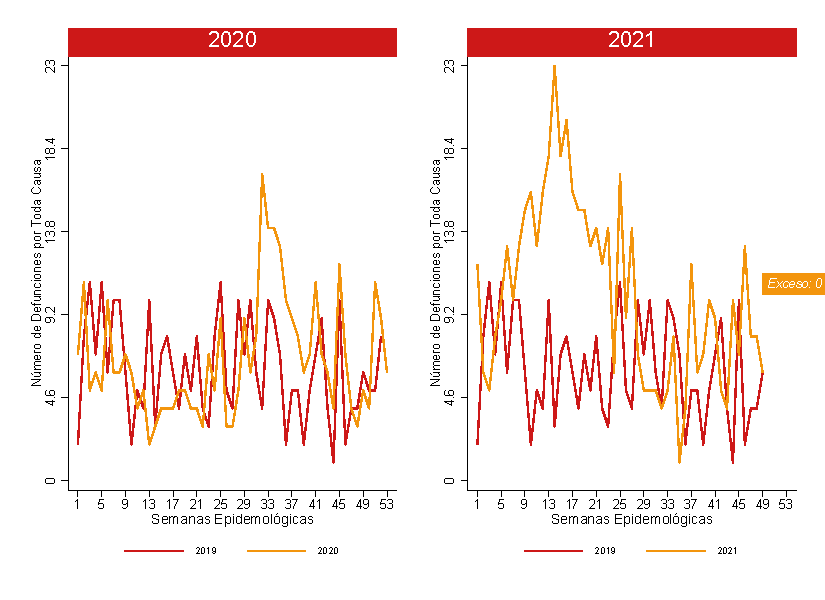
\includegraphics[width=0.7\linewidth]{../figuras/exceso_2.pdf}
			\end{center}
			{\footnotesize {Fuente de datos: SINADEF.}}
		\end{figure}
		
		% Canas
		\clearpage
		
		\subsection*{Provincia de Canas}
		\noindent La Figura \ref{fig:inc_mort_canas} se evidencia un ascenso sostenido de la tasa de incidencia a partir de la SE 01 del año 2022, junto con este ascenso se observa un incremento de la tasa de mortalidad para la misma semana. 
		\noindent La Figura \ref{fig:positividad_canas} muestra una tendencia al ascenso de la positividad de ambas pruebas a partir de la misma semana del incremento de incidencia. 
		
		La Figura \ref{fig:exceso_canas} muestra que hay un exceso negativo de menos una defunción respecto al año 2019.
		
		\begin{figure}[h]
			\caption{Tasa de Incidencia y Mortalidad Comparativa en la Provincia de Canas hasta la SE 07-2022.}\label{fig:inc_mort_canas}
			\begin{center}
				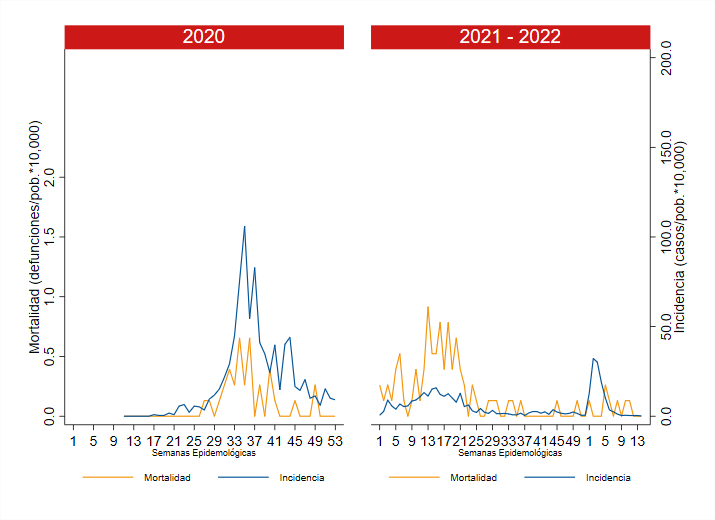
\includegraphics[width=0.7\linewidth]{../figuras/incidencia_mortalidad_20_21_3.png}
			\end{center}
			{\footnotesize {Fuente de datos: NOTICOVID, SISCOVID, SINADEF.}}
		\end{figure}
		
		\begin{figure}[h]
			\caption{Tasa de Positividad de Prueba Molecular y Antigénica Comparativa en la Provincia de Canas hasta la SE 07-2022.}\label{fig:positividad_canas}
			\begin{center}
				\includegraphics[width=0.7\linewidth]{../figuras/positividad_20_21_3.png}
			\end{center}
			{\footnotesize {Fuente de datos: NOTICOVID, SISCOVID.}}
		\end{figure}
		
		\begin{figure}[h]
			\caption{Exceso de Defunciones Comparativo en la Provincia de Canas hasta la SE 07-2022.}\label{fig:exceso_canas}
			\begin{center}
				\includegraphics[width=0.7\linewidth]{../figuras/exceso_3.pdf}
			\end{center}
			{\footnotesize {Fuente de datos: SINADEF.}}
		\end{figure}
		
		% Calca
		\clearpage
		
		\subsection*{Provincia de Calca}
		\noindent Las figuras de abajo (Figura \ref{fig:inc_mort_calca}, \ref{fig:positividad_calca}) muestran el comportamiento de la tasa de incidencia, mortalidad y  positividad. Con respecto a la tasa de incidencia, se evidencia un ascenso sostenido a partir de la SE 01 del año 2022, mientras que la tasa de mortalidad se ha mantenido constante con cero defunciones. 
		
		En la Figura \ref{fig:exceso_calca} se muestra que hay un exceso de menos 6 defunciones (exceso negativo) respecto al año 2019.
		
		\begin{figure}[h]
			\caption{Tasa de Incidencia y Mortalidad Comparativa en la Provincia de Calca hasta la SE 07-2022.}\label{fig:inc_mort_calca}
			\begin{center}
				\includegraphics[width=0.7\linewidth]{../figuras/incidencia_mortalidad_20_21_4.png}
			\end{center}
			{\footnotesize {Fuente de datos: NOTICOVID, SISCOVID, SINADEF.}}
		\end{figure}
		
		\begin{figure}[h]
			\caption{Tasa de Positividad de Prueba Molecular y Antigénica Comparativa en la Provincia de Calca hasta la SE 07-2022.}\label{fig:positividad_calca}
			\begin{center}
				\includegraphics[width=0.7\linewidth]{../figuras/positividad_20_21_4.png}
			\end{center}
			{\footnotesize {Fuente de datos: NOTICOVID, SISCOVID.}}
		\end{figure}
		
		\begin{figure}[h]
			\caption{Exceso de Defunciones Comparativo en la Provincia de Calca hasta la SE 07-2022.}\label{fig:exceso_calca}
			\begin{center}
				\includegraphics[width=0.7\linewidth]{../figuras/exceso_4.pdf}
			\end{center}
			{\footnotesize {Fuente de datos: SINADEF.}}
		\end{figure}
		
		% Canas
		\clearpage
		
		\subsection*{Provincia de Canchis}
		\noindent La Figura \ref{fig:inc_mort_canchis} se evidencia un ascenso sostenido de la tasa de incidencia a partir de la SE 01 del año 2022, así como un ascenso en la tasa de mortalidad. 
		\noindent La Figura \ref{fig:positividad_canchis} muestra el ascenso de ambas tasas de positividad tanto antigénicas y moleculares desde la SE 01 del 2022.
		
		En la Figura \ref{fig:exceso_canchis} se muestra que hay un exceso de menos 15 defunciones (exceso negativo) respecto al año 2019.
		
		\begin{figure}[h]
			\caption{Tasa de Incidencia y Mortalidad Comparativa en la Provincia de Canchis hasta la SE 07-2022.}\label{fig:inc_mort_canchis}
			\begin{center}
				\includegraphics[width=0.7\linewidth]{../figuras/incidencia_mortalidad_20_21_5.png}
			\end{center}
			{\footnotesize {Fuente de datos: NOTICOVID, SISCOVID, SINADEF.}}
		\end{figure}
		
		\begin{figure}[h]
			\caption{Tasa de Positividad de Prueba Molecular y Antigénica Comparativa en la Provincia de Canchis hasta la SE 07-2022.}\label{fig:positividad_canchis}
			\begin{center}
				\includegraphics[width=0.7\linewidth]{../figuras/positividad_20_21_5.png}
			\end{center}
			{\footnotesize {Fuente de datos: NOTICOVID, SISCOVID.}}
		\end{figure}
		
		\begin{figure}[h]
			\caption{Exceso de Defunciones Comparativo en la Provincia de Canchis hasta la SE 07-2022.}\label{fig:exceso_canchis}
			\begin{center}
				\includegraphics[width=0.7\linewidth]{../figuras/exceso_5.pdf}
			\end{center}
			{\footnotesize {Fuente de datos: SINADEF.}}
		\end{figure}
		
		\clearpage
		
		% Chumbivilcas
		\subsection*{Provincia de Chumbivilcas}
		\noindent La Figura \ref{fig:inc_mort_chumbivilcas} se evidencia un ascenso sostenido de la tasa de incidencia a partir de la SE 01 del año 2022, asociado a un incremento de muertes para la SE 02 del 2022.  
		\noindent La Figura \ref{fig:positividad_chumbivilcas} muestra una tendencia al ascenso de ambas tasas de positividad desde la SE 01 del año 2022. 
		
		En la Figura \ref{fig:exceso_chumbivilcas} se muestra que hay un exceso de menos 5 defunciones (exceso negativo) respecto al año 2019.
		
		\begin{figure}[h]
			\caption{Tasa de Incidencia y Mortalidad Comparativa en la Provincia de Chumbivilcas hasta la SE 07-2022.}\label{fig:inc_mort_chumbivilcas}
			\begin{center}
				\includegraphics[width=0.7\linewidth]{../figuras/incidencia_mortalidad_20_21_6.png}
			\end{center}
			{\footnotesize {Fuente de datos: NOTICOVID, SISCOVID, SINADEF.}}
		\end{figure}
		
		\begin{figure}[h]
			\caption{Tasa de Positividad de Prueba Molecular y Antigénica Comparativa en la Provincia de Chumbivilcas 2020 hasta la SE 07-2022.}\label{fig:positividad_chumbivilcas}
			\begin{center}
				\includegraphics[width=0.7\linewidth]{../figuras/positividad_20_21_6.png}
			\end{center}
			{\footnotesize {Fuente de datos: NOTICOVID, SISCOVID.}}
		\end{figure}
		
		\begin{figure}[h]
			\caption{Exceso de Defunciones Comparativo en la Provincia de Chumbivilcas hasta la SE 07-2022.}\label{fig:exceso_chumbivilcas}
			\begin{center}
				\includegraphics[width=0.7\linewidth]{../figuras/exceso_6.pdf}
			\end{center}
			{\footnotesize {Fuente de datos: SINADEF.}}
		\end{figure}
		
		% Cusco
		\clearpage
		
		\subsection*{Provincia de Cusco}
		\noindent La Figura \ref{fig:inc_mort_cusco} se evidencia un ascenso sostenido de la tasa de incidencia a partir de la SE 01 del año 2022, mientras que el ascenso de la tasa de mortalidad inicia en la SE 02 del 2022.   
		\noindent La  Figura \ref{fig:positividad_cusco} muestra el mismo comportamiento para las tasas de positividad de ambas pruebas a partir de la SE 01 del 2022. 
	
	En la Figura \ref{fig:exceso_cusco} se muestra que hay exceso de menos 29 defunciones (exceso negativo) respecto al año 2019.
		
		\begin{figure}[h]
			\caption{Tasa de Incidencia y Mortalidad Comparativa en la Provincia de Cusco hasta la SE 07-2022.}\label{fig:inc_mort_cusco}
			\begin{center}
				\includegraphics[width=0.7\linewidth]{../figuras/incidencia_mortalidad_20_21_7.png}
			\end{center}
			{\footnotesize {Fuente de datos: NOTICOVID, SISCOVID, SINADEF.}}
		\end{figure}
		
		\begin{figure}[h]
			\caption{Tasa de Positividad de Prueba Molecular y Antigénica Comparativa en la Provincia de Cusco hasta la SE 07-2022.}\label{fig:positividad_cusco}
			\begin{center}
				\includegraphics[width=0.7\linewidth]{../figuras/positividad_20_21_7.png}
			\end{center}
			{\footnotesize {Fuente de datos: NOTICOVID, SISCOVID.}}
		\end{figure}
		
		\begin{figure}[h]
			\caption{Exceso de Defunciones Comparativo en la Provincia de Cusco hasta la SE 07-2022.}\label{fig:exceso_cusco}
			\begin{center}
				\includegraphics[width=0.7\linewidth]{../figuras/exceso_7.pdf}
			\end{center}
			{\footnotesize {Fuente de datos: SINADEF.}}
		\end{figure}
		
		% Espinar
		\clearpage
		
		\subsection*{Provincia de Espinar}
		\noindent Las figuras de abajo (Figura \ref{fig:inc_mort_espinar}, \ref{fig:positividad_espinar}) muestran el comportamiento de la tasa de incidencia, mortalidad y positividad. Se evidencia un ascenso sostenido de la tasa de incidencia a partir de la SE 01 del año 2022.
		
		En la Figura \ref{fig:exceso_espinar} se muestra que hay exceso de menos 2 defunciones (exceso negativo) respecto al año 2019.
		
		\begin{figure}[h]
			\caption{Tasa de Incidencia y Mortalidad Comparativa en la Provincia de Espinar hasta la SE 07-2022.}\label{fig:inc_mort_espinar}
			\begin{center}
				\includegraphics[width=0.7\linewidth]{../figuras/incidencia_mortalidad_20_21_8.png}
			\end{center}
			{\footnotesize {Fuente de datos: NOTICOVID, SISCOVID, SINADEF.}}
		\end{figure}
		
		\begin{figure}[h]
			\caption{Tasa de Positividad de Prueba Molecular y Antigénica Comparativa en la Provincia de Espinar hasta la SE 07-2022.}\label{fig:positividad_espinar}
			\begin{center}
				\includegraphics[width=0.7\linewidth]{../figuras/positividad_20_21_8.png}
			\end{center}
			{\footnotesize {Fuente de datos: NOTICOVID, SISCOVID.}}
		\end{figure}
		
		\begin{figure}[h]
			\caption{Exceso de Defunciones Comparativo en la Provincia de Espinar hasta la SE 07-2022.}\label{fig:exceso_espinar}
			\begin{center}
				\includegraphics[width=0.7\linewidth]{../figuras/exceso_8.pdf}
			\end{center}
			{\footnotesize {Fuente de datos: SINADEF.}}
		\end{figure}
		
		% La Convención
		\clearpage
		
		\subsection*{Provincia de La Convención}
		\noindent Las figuras inferiores (Figura \ref{fig:inc_mort_laconv}, \ref{fig:positividad_laconv}) muestran el comportamiento de la tasa de incidencia y mortalidad. Se evidencia un ascenso sostenido de la tasa de incidencia a partir de la SE 01 del año 2022, así como en la tasa de mortalidad. 

		
	En la Figura \ref{fig:exceso_laconv} se muestra que hay exceso de menos 17 defunciones (exceso negativo) respecto al año 2019.
		
		\begin{figure}[h]
			\caption{Tasa de Incidencia y Mortalidad Comparativa en la Provincia de La Convención hasta la SE 07-2022.}\label{fig:inc_mort_laconv}
			\begin{center}
				\includegraphics[width=0.7\linewidth]{../figuras/incidencia_mortalidad_20_21_9.png}
			\end{center}
			{\footnotesize {Fuente de datos: NOTICOVID, SISCOVID, SINADEF.}}
		\end{figure}
		
		\begin{figure}[h]
			\caption{Tasa de Positividad de Prueba Molecular y Antigénica Comparativa en la Provincia de La Convención hasta la SE 07-2022.}\label{fig:positividad_laconv}
			\begin{center}
				\includegraphics[width=0.7\linewidth]{../figuras/positividad_20_21_9.png}
			\end{center}
			{\footnotesize {Fuente de datos: NOTICOVID, SISCOVID.}}
		\end{figure}
		
		\begin{figure}[h]
			\caption{Exceso de Defunciones Comparativo en la Provincia de La Convención hasta la SE 07-2022.}\label{fig:exceso_laconv}
			\begin{center}
				\includegraphics[width=0.7\linewidth]{../figuras/exceso_9.pdf}
			\end{center}
			{\footnotesize {Fuente de datos: SINADEF.}}
		\end{figure}
		
		% Paruro
		\clearpage
		
		\subsection*{Provincia de Paruro}
		\noindent Las figuras de abajo (Figura \ref{fig:inc_mort_paruro}, \ref{fig:positividad_paruro}) muestran el comportamiento de la tasa de incidencia, mortalidad y positividad. La tasa de incidencia ha presentando un pendiente en ascenso a partir de la SE 01 del 2022, mientras que la tasa de mortalidad muestra un ascenso a partir de la SE 02 del 2022.  
	 
	 En la Figura \ref{fig:exceso_paruro} se muestra un exceso de menos 4 defunciones(exceso negativo) con respecto al año 2019.
		
		\begin{figure}[h]
			\caption{Tasa de Incidencia y Mortalidad Comparativa en la Provincia de Paruro, hasta la SE 07-2022.}\label{fig:inc_mort_paruro}
			\begin{center}
				\includegraphics[width=0.7\linewidth]{../figuras/incidencia_mortalidad_20_21_10.png}
			\end{center}
			{\footnotesize {Fuente de datos: NOTICOVID, SISCOVID, SINADEF.}} 
		\end{figure}
		
		\begin{figure}[h]
			\caption{Tasa de Positividad de Prueba Molecular y Antigénica Comparativa en la Provincia de Paruro hasta la SE 07-2022.}\label{fig:positividad_paruro}
			\begin{center}
				\includegraphics[width=0.7\linewidth]{../figuras/positividad_20_21_10.png}
			\end{center}
			{\footnotesize {Fuente de datos: NOTICOVID, SISCOVID.}}
		\end{figure}
		
		\begin{figure}[h]
			\caption{Exceso de Defunciones Comparativo en la Provincia de Paruro hasta la SE 07-2022.}\label{fig:exceso_paruro}
			\begin{center}
				\includegraphics[width=0.7\linewidth]{../figuras/exceso_10.pdf}
			\end{center}
			{\footnotesize {Fuente de datos: SINADEF.}}
		\end{figure}
		
		
		% Paucartambo
		\clearpage
		
		\subsection*{Provincia de Paucartambo}
		\noindent Las figuras de abajo (Figura \ref{fig:inc_mort_paucartam}, \ref{fig:positividad_paucartam}) muestran el comportamiento de la tasa de incidencia, mortalidad y positividad. Se evidencia el ascenso de ambas tasas, iniciando el ascenso en la SE 01 del año 2022. 
	En la Figura \ref{fig:exceso_paucartam} se muestra un exceso de menos 4 defunciones (exceso negativo) respecto al año 2019.
		
		\begin{figure}[h]
			\caption{Tasa de Incidencia y Mortalidad Comparativa en la Provincia de Paucartambo hasta la SE 07-2022.}\label{fig:inc_mort_paucartam}
			\begin{center}
				\includegraphics[width=0.7\linewidth]{../figuras/incidencia_mortalidad_20_21_11.png}
			\end{center}
			{\footnotesize {Fuente de datos: NOTICOVID, SISCOVID, SINADEF.}}
		\end{figure}
		
		\begin{figure}[h]
			\caption{Tasa de Positividad de Prueba Molecular y Antigénica Comparativa en la Provincia de Paucartambo hasta la SE 07-2022.}\label{fig:positividad_paucartam}
			\begin{center}
				\includegraphics[width=0.7\linewidth]{../figuras/positividad_20_21_11.png}
			\end{center}
			{\footnotesize {Fuente de datos: NOTICOVID, SISCOVID.}}
		\end{figure}
		
		\begin{figure}[h]
			\caption{Exceso de Defunciones Comparativo en la Provincia de Paucartambo hasta la SE 07-2022.}\label{fig:exceso_paucartam}
			\begin{center}
				\includegraphics[width=0.7\linewidth]{../figuras/exceso_11.pdf}
			\end{center}
			{\footnotesize {Fuente de datos: SINADEF.}}
		\end{figure}
		
		% Quispicanchi
		\clearpage
		
		\subsection*{Provincia de Quispicanchi}
		\noindent Las figuras de abajo (Figura \ref{fig:inc_mort_quisp}, \ref{fig:positividad_quisp}) muestran el comportamiento de la tasa de incidencia, mortalidad y positividad. Con respecto a la tasa de incidencia se evidencia un incremento marcado a partir de la SE 01 del año 2022, mientras que la tasa de mortalidad muestra un ligero ascenso.   

		
	En la Figura \ref{fig:exceso_quisp} se muestra que hay un exceso de menos 7 defunciones (exceso negativo) respecto al año 2019.
		
		\begin{figure}[h]
			\caption{Tasa de Incidencia y Mortalidad Comparativa en la Provincia de Quispicanchi hasta la SE 07-2022.}\label{fig:inc_mort_quisp}
			\begin{center}
				\includegraphics[width=0.7\linewidth]{../figuras/incidencia_mortalidad_20_21_12.png}
			\end{center}
			{\footnotesize {Fuente de datos: NOTICOVID, SISCOVID, SINADEF.}}
		\end{figure}
		
		\begin{figure}[h]
			\caption{Tasa de Positividad de Prueba Molecular y Antigénica Comparativa en la Provincia de Quispicanchi hasta la SE 07-2022.}\label{fig:positividad_quisp}
			\begin{center}
				\includegraphics[width=0.7\linewidth]{../figuras/positividad_20_21_12.png}
			\end{center}
			{\footnotesize {Fuente de datos: NOTICOVID, SISCOVID.}}
		\end{figure}
		
		\begin{figure}[h]
			\caption{Exceso de Defunciones Comparativo en la Provincia de Quispicanchis hasta la SE 07-2022.}\label{fig:exceso_quisp}
			\begin{center}
				\includegraphics[width=0.7\linewidth]{../figuras/exceso_12.pdf}
			\end{center}
			{\footnotesize {Fuente de datos: SINADEF.}}
		\end{figure}
		
		% Urubamba
		\clearpage
		
		\subsection*{Provincia de Urubamba}
		\noindent Las figuras de abajo (Figura \ref{fig:inc_urub}, \ref{fig:positividad_urub}) muestran el comportamiento de la tasa de incidencia, mortalidad y positividad. Con respecto a la tasa de incidencia se evidencia un incremento marcado a partir de la SE 01 del año 2022, mientras que la tasa de mortalidad comienza a ascender desde la SE 02 del año 2022. 
	
		En la Figura \ref{fig:exceso_urub} se muestra un exceso de menos diez defunciones (exceso negativo) respecto al año 2019.
		
		\begin{figure}[h]
			\caption{Tasa de Incidencia y Mortalidad Comparativa en la Provincia de Urubamba hasta la SE 07-2022.}\label{fig:inc_urub}
			\begin{center}
				\includegraphics[width=0.7\linewidth]{../figuras/incidencia_mortalidad_20_21_13.png}
			\end{center}
			{\footnotesize {Fuente de datos: NOTICOVID, SISCOVID, SINADEF.}}
		\end{figure}
		
		\begin{figure}[h]
			\caption{Tasa de Positividad de Prueba Molecular y Antigénica Comparativa en la Provincia de Urubamba hasta la SE 07-2022.}\label{fig:positividad_urub}
			\begin{center}
				\includegraphics[width=0.7\linewidth]{../figuras/positividad_20_21_13.png}
			\end{center}
			{\footnotesize {Fuente de datos: NOTICOVID, SISCOVID.}}
		\end{figure}
		
		\begin{figure}[h]
			\caption{Exceso de Defunciones Comparativo en la Provincia de Urubamba hasta la SE 07-2022.}\label{fig:exceso_urub}
			\begin{center}
				\includegraphics[width=0.7\linewidth]{../figuras/exceso_13.pdf}
			\end{center}
			{\footnotesize {Fuente de datos: SINADEF.}}
		\end{figure}
		
		\clearpage
%---------------------------------------------------------------------------
		% CAPÍTULO: VARIANTES DE COVID-19
		%---------------------------------------------------------------------------
		%insertar el cover del capitulo
		\includepdf[pages={1}]{../editorial/6.pdf}
		\clearpage
		
		\section* {Variantes de COVID-19 en la Región Cusco}
		\addcontentsline{toc}{chapter}{Variantes de COVID-19}
		\noindent La aparición de la variante ómicron ha generado la tercera ola de COVID-19 en el Perú debido a su gran transmisibilidad. En la Figura \ref{fig:variantes} se observa que en la región Cusco, la variante ómicron (87$\%$) ha desplazado a la variante Delta (9$\%$) en el secuenciamiento genético semanal durante el mes de enero, se espera que esta tendencia continúe a lo largo de la tercera ola. 
		Hasta el 22 de enero del 2022 se secuenciaron 349 muestras a nivel de la región de Cusco 
		encontrándose las variantes beta (B.1.1.348), gamma (P.1, P.1.7), lambda (C.37), delta (B.1617.2), mu y ómicron (BA.1.1). 
		La vigilancia genómica es realizada en colaboración con 4 instituciones externas a GERESA-Cusco.
						
		\begin{figure}[h]
			\caption{Prevalencia de las variantes de SARS Cov-2 aisladas en la región de Cusco, hasta Febrero-2022. }\label{fig:variantes}
			\begin{center}
				\includegraphics[width=0.85\linewidth]{../figuras/variantes.pdf}
			\end{center}
			{\footnotesize {Fuente de datos: INS-NETLAB, UPCH, UNSAAC}}
		\end{figure}
		
	Asímismo, la Figura \ref{fig:mapa_variantes} muestra las variantes de COVID-19 aisladas por zonas. Aunque las muestras secuenciadas como variante ómicron fueron principalmente de la provincia Cusco, se estima que esta variante está ampliamente distribuida en la región debido a su gran transmisibilidad. 
	
			\begin{figure}[h]
				\caption{Distribución provincial de las variantes de SARS-CoV-2 aisladas en la Región Cusco hasta la SE 07-2022.}
				\label{fig:mapa_variantes}
				\centering
				\begin{subfigure}[b]{0.40\textwidth}
					\centering
					\includegraphics[width=\textwidth]{../figuras/variantes_provincial_lambda.pdf}
					\caption{Variante Lambda}
					%\label{fig:}
				\end{subfigure}
				\hfill
				\begin{subfigure}[b]{0.40\textwidth}
					\centering
					\includegraphics[width=\textwidth]{../figuras/variantes_provincial_gamma.pdf}
					\caption{Variante Gamma}
					%\label{fig:70 a 79 años}
				\end{subfigure}
							
				\begin{subfigure}[b]{0.40\textwidth}
					\centering
					\includegraphics[width=\textwidth]{../figuras/variantes_provincial_delta.pdf}
					\caption{Variante Delta}
					%\label{fig:60 a 69 años}
				\end{subfigure}
			\vspace{0.5mm}
			\hspace{25mm}
			\begin{subfigure}[b]{0.40\textwidth}
				\centering
				\includegraphics[width=\textwidth]{../figuras/variantes_provincial_omicron.pdf}
				\caption{Variante Ómicron}
				%\label{fig:60 a 69 años}
			\end{subfigure}
			\end{figure}

\clearpage
%---------------------------------------------------------------------------
% CAPÍTULO: DEFUNCIONES CERO
%-------------------------------------------

%insertar el cover del capitulo
\includepdf[pages={1}]{../editorial/7.pdf}
\clearpage
	\section*{Semanas con Cero Defunciones por COVID-19 por Semana a Nivel Provincial}\addcontentsline{toc}{chapter}{Defunciones Cero}
	
\noindent En la tabla inferior se muestra las provincias con cero defunciones reportadas (casillas en amarillo) por cada semana epidemiológica. Durante la primera semana de enero se han reportado muertes en las provincias de Cusco, Canchis, Espinar y La Convención. Para la tercera semana siete de las trece provincias reportaron muertes por COVID-19, con mayor número en la provincia de Cusco, Chumbivilcas, La Convención y Quispicanchis. Es importante recalcar que provincia de Acomayo se mantiene con cero defunciones por COVID-19 desde la SE 47 del año 2021.
	\begin{table}[h]		\caption{Defunciones Cero por COVID-19 a nivel Provincial hasta la SE 07-2022.}
		\resizebox{\textwidth}{!}{%
			\begin{tabular}{lccccccccc}
	\textbf{}              	  
	& \multicolumn{1}{l}{}                        
	& \multicolumn{1}{l}{}      
	& \multicolumn{1}{l}{}                         
	& \multicolumn{1}{l}{}                         
	& \multicolumn{1}{l}{}                         
	& \multicolumn{1}{l}{}                        
	& \multicolumn{1}{l}{}                         
	& \multicolumn{1}{l}{} \\                   
	\textbf{}                                                                 				
	&\textbf{SE-31} 							
	&\textbf{SE-32}						
	&\textbf{SE-33}								
	&\textbf{SE-34}					
	&\textbf{SE-35}								
	&\textbf{SE-36}
	&\textbf{SE-37}
	&\textbf{SE-38}\\							
	\textbf{}              	  																
	&\textbf{31jul-06ago}						
	&\textbf{07ago-13ago}						
	&\textbf{14ago-20ago}						
	&\textbf{21ago-27ago}						
	&\textbf{28ago-03sep}
	&\textbf{04sep-10sep}
	&\textbf{11sep-17sep} 
	&\textbf{18sep-24sep} \\
	\textbf{Acomayo}                        												
	&\cellcolor[HTML]{FCC46C}
	&\cellcolor[HTML]{FCC46C}					
	&\cellcolor[HTML]{FCC46C}
	&\cellcolor[HTML]{FCC46C}					
	&\cellcolor[HTML]{FCC46C}
	&\cellcolor[HTML]{FCC46C} 
	&\cellcolor[HTML]{FCC46C}
	&\cellcolor[HTML]{FCC46C}\\
	\textbf{Anta}                                                  				
	&1											
	&\cellcolor[HTML]{FCC46C}					
	&\cellcolor[HTML]{FCC46C}					
	&\cellcolor[HTML]{FCC46C}					
	&\cellcolor[HTML]{FCC46C}
	&\cellcolor[HTML]{FCC46C}	
	&\cellcolor[HTML]{FCC46C}
	&\cellcolor[HTML]{FCC46C}\\					
	\textbf{Calca}      				       									
	&\cellcolor[HTML]{FCC46C}					
	&1											
	&\cellcolor[HTML]{FCC46C}					
	&1											
	&\cellcolor[HTML]{FCC46C}
	&1
	&1
	&\cellcolor[HTML]{FCC46C}\\          			
	\textbf{Canas}                              									
	&\cellcolor[HTML]{FCC46C}
	&1											
	&1
	&\cellcolor[HTML]{FCC46C}					
	&\cellcolor[HTML]{FCC46C}
	&\cellcolor[HTML]{FCC46C}	
	&\cellcolor[HTML]{FCC46C}
	&\cellcolor[HTML]{FCC46C}\\	
	\textbf{Canchis}    						
	&1			
	&\cellcolor[HTML]{FCC46C}					
	&\cellcolor[HTML]{FCC46C}			
	&\cellcolor[HTML]{FCC46C}					
	&1
	&1
	&\cellcolor[HTML]{FCC46C}
	&\cellcolor[HTML]{FCC46C}\\											
	\textbf{Chumbivilcas}                      									
	&\cellcolor[HTML]{FCC46C}
	&\cellcolor[HTML]{FCC46C}					
	&\cellcolor[HTML]{FCC46C}
	&\cellcolor[HTML]{FCC46C}					
	&1
	&\cellcolor[HTML]{FCC46C}
	&1
	&1\\
	\textbf{Cusco}      															
	&2		
	&3											
	&2
	&4											
	&1
	&1
	&\cellcolor[HTML]{FCC46C}
	&\cellcolor[HTML]{FCC46C}\\								
	\textbf{Espinar}       					             							
	&\cellcolor[HTML]{FCC46C}					
	&\cellcolor[HTML]{FCC46C}
	&\cellcolor[HTML]{FCC46C}					
	&\cellcolor[HTML]{FCC46C}
	&\cellcolor[HTML]{FCC46C}					
	&\cellcolor[HTML]{FCC46C}
	&\cellcolor[HTML]{FCC46C}
	&\cellcolor[HTML]{FCC46C}\\	
	\textbf{La Convención}       
	&3											
	&1											
	&2											
	&1											
	&3
	&\cellcolor[HTML]{FCC46C}
	&\cellcolor[HTML]{FCC46C}
	&\cellcolor[HTML]{FCC46C}\\	
	\textbf{Paruro}                            					
	&\cellcolor[HTML]{FCC46C}					
	&\cellcolor[HTML]{FCC46C}					
	&\cellcolor[HTML]{FCC46C}					
	&\cellcolor[HTML]{FCC46C}					
	&\cellcolor[HTML]{FCC46C}
	&\cellcolor[HTML]{FCC46C} 					
	&\cellcolor[HTML]{FCC46C}
	&\cellcolor[HTML]{FCC46C}\\
	\textbf{Paucartambo}               		                       					
	&\cellcolor[HTML]{FCC46C}					
	&\cellcolor[HTML]{FCC46C}
	&\cellcolor[HTML]{FCC46C}					
	&\cellcolor[HTML]{FCC46C}
	&\cellcolor[HTML]{FCC46C}					
	&\cellcolor[HTML]{FCC46C}
	&\cellcolor[HTML]{FCC46C}
	&\cellcolor[HTML]{FCC46C}\\
	\textbf{Quispicanchi}          	      				
	&1											
	&\cellcolor[HTML]{FCC46C}					
	&1											
	&\cellcolor[HTML]{FCC46C}					
	&1
	&\cellcolor[HTML]{FCC46C}
	&\cellcolor[HTML]{FCC46C}
	&\cellcolor[HTML]{FCC46C}\\
	\textbf{Urubamba}  					
	&1											
	&\cellcolor[HTML]{FCC46C}					
	&\cellcolor[HTML]{FCC46C}					
	&1											
	&1	
	&\cellcolor[HTML]{FCC46C}
	&\cellcolor[HTML]{FCC46C}
	&\cellcolor[HTML]{FCC46C}\\						
	&\multicolumn{1}{l}{}                       &\multicolumn{1}{l}{}            &\multicolumn{1}{l}{}                         
	&\multicolumn{1}{l}{}                       &\multicolumn{1}{l}{}            &\multicolumn{1}{l}{}                       &\multicolumn{1}{l}{}                       &\multicolumn{1}{l}{}            			    
\end{tabular}
		}
		{\footnotesize {Fuente de datos: SINADEF.}}
	\end{table}
\pagebreak

%---------------------------------------------------------------------------
% CAPÍTULO: AGRADECIMIENTOS
%---------------------------------------------------------------------------
	\section*{Agradecimientos}
	\addcontentsline{toc}{chapter}{Agradecimientos}
		
	\centering
		{\large El presente Boletín Epidemiológico COVID-19 se ha elaborado gracias a la información y esfuerzo conjunto de los Equipos de Inteligencia Sanitaria de los Hospitales y Redes de la GERESA Cusco:

		\vspace{0.5cm}
		\noindent
		\begin{minipage}[t]{.45\textwidth}
			\centering
			Hospital Regional del Cusco \\
			M.S.P. Marina Ochoa Linares \vspace{0.5cm}\\
			Hospital Antonio Lorena \\
			Dr. Homero Dueñas \vspace{.5cm}\\
			Hospital Nacional Adolfo Guevara Velasco\\
			M.S.P. Lucio Velasquez Cuentas \vspace{.5cm}\\
			Red de Salud Norte \\
			M.C. Guido Giraldo Alencastre\vspace{0.5cm}\\
			Red de Salud Sur\\
			Lic. Luz Marina Bernable Villasante \vspace{0.5cm}\\	
		\end{minipage}
		\hfill
		\noindent
		\begin{minipage}[t]{.45\textwidth}
			\centering
			Red de Salud La Convención\\
			Dr. David Coanqui Pacori\vspace{0.5cm}\\
			Red de Salud Chumbivilcas\\
			Lic. Eduarda Benito Calderón \vspace{.5cm}\\
			Red de Salud Canas Canchis Espinar\\
			MC. Heber Jaime Quispe Jihuallanca \vspace{.5cm}\\
			Red de Salud Kimbiri Pichari \\
			Lic. Fiorella Castillo Tinoco\vspace{0.5cm}\\	
		\end{minipage}
%---------------------------------------------------------------------------
% CAPÍTULO: AGRADECIMIENTOS
%---------------------------------------------------------------------------
	\chapter*{Diseño y Edición}
	\addcontentsline{toc}{chapter}{Diseño y Edición}
	\begin{center}
	
	% Como siempre, por orden alfabético del apellid0
	
	MSC. Fátima R. Concha Velasco
	
	M.C. Ana Gabriela Eulalia Moncada Arias 
	
	Ing. Joel Wilfredo Sumerente Ayerbe
	\end{center}

	%insertar la última página
	\includepdf[pages={1}]{../editorial/pagina_final.pdf}
	\clearpage
	
\end{document}